\documentclass[xcolor=svgnames,9pt,english,aspectratio=169,t]{beamer}
%\documentclass[xcolor=svgnames,9pt,english,handout,aspectratio=169,t]{beamer}
\newcommand{\handout}{0}

% =====================================================================
% POLI 450A (2026) --- shared TEMPLATE layer.
%
% Input from each lecture near the top of its file, BEFORE
% ../course_theme.tex (metropolis must be selected before the course
% palette overrides it):
%
%   \documentclass[xcolor=svgnames,9pt,english,aspectratio=169]{beamer}
%   \newcommand{\handout}{0}
%   % =====================================================================
% POLI 450A (2026) --- shared TEMPLATE layer.
%
% Input from each lecture near the top of its file, BEFORE
% ../course_theme.tex (metropolis must be selected before the course
% palette overrides it):
%
%   \documentclass[xcolor=svgnames,9pt,english,aspectratio=169]{beamer}
%   \newcommand{\handout}{0}
%   % =====================================================================
% POLI 450A (2026) --- shared TEMPLATE layer.
%
% Input from each lecture near the top of its file, BEFORE
% ../course_theme.tex (metropolis must be selected before the course
% palette overrides it):
%
%   \documentclass[xcolor=svgnames,9pt,english,aspectratio=169]{beamer}
%   \newcommand{\handout}{0}
%   \input{../course_preamble.tex}
%   \input{../course_theme.tex}
%   \graphicspath{{./}{./figs/}}
%   \title[Short title]{450A Political Methodology I}
%   \subtitle{Lecture N: ...}
%
% Modeled on the 2026 Northwestern workshop template
% (Teaching/PanelData/_latex/2026/202608_Northwestern/workshop_preamble.tex).
%
% SCOPE: theme, beamer layout, packages, the roadmap hooks, and --- unlike
% the Northwestern decks --- the notation macros. The 450A lectures
% grew from one common ancestor, so their macro blocks agree wherever they
% overlap; merging them is safe. Three points where they had drifted are
% resolved here, and each is flagged inline below.
% =====================================================================

\usetheme{metropolis}
\metroset{sectionpage=none, subsectionpage=none, numbering=none}
\setbeamertemplate{navigation symbols}{}

\setbeamersize{text margin left=5mm, text margin right=5mm}
\setbeamertemplate{itemize/enumerate body begin}{\leftmargini=1.5em\relax}
\setbeamertemplate{itemize/enumerate subbody begin}{\leftmarginii=1.5em\relax}
\setbeamertemplate{itemize/enumerate subsubbody begin}{\leftmarginiii=1.5em\relax}

% ----------------------------------------------------------- top alignment
% Every deck passes the t class option, so beamer applies the frame key
% below to every frame (explicit [plain,c] frames — title page, roadmaps —
% stay centered). Beamer's stock t key puts a rigid .2cm pad above the
% content; frames sized to this template's full-height ceilings then run
% Overfull \vbox by up to that pad. Same key as beamerbaseframe.sty, with
% one change: the pad may shrink to zero when the frame is full.
\makeatletter
\define@key{beamerframe}{t}[true]{% top
  \beamer@frametopskip=.2cm plus .5\paperheight minus .2cm\relax%
  \beamer@framebottomskip=0pt plus 1fill\relax%
  \beamer@frametopskipautobreak=\beamer@frametopskip\relax%
  \beamer@framebottomskipautobreak=\beamer@framebottomskip\relax%
}

% ------------------------------------------------- slide-top check (2026-10-11)
% A slide whose content is too tall for the frame is squeezed: the pad above
% shrinks and its content starts higher than on other slides, so a figure
% "wobbles" when the class steps from one slide to the next (Lecture 4-1,
% slides 1-2, 2026-10-11). The marker below records where each slide's
% content starts (a whatsit: it adds no space and moves nothing).
% `python3 ../check_slides.py lec<N>` then lists every slide that starts
% higher than the deck's normal position. That list must be empty.
% Recorded per slide: page, frame number, content-top y (sp), the room left
% below the title bar, and P for a plain frame (title page, roadmaps).
\providecommand\slidetop[5]{}
\AtBeginDocument{\immediate\write\@auxout{\string\providecommand\string\slidetop[5]{}}}
\def\beamer@markframetop{%
  \pdfsavepos
  \edef\beamer@marktmp{\noexpand\write\noexpand\@auxout{\string\slidetop
    {\noexpand\thepage}{\noexpand\insertframenumber}{\noexpand\the\noexpand\pdflastypos}%
    {\number\beamer@frametextheight}{\ifbeamer@plainframe P\else N\fi}}}%
  \beamer@marktmp}
\RequirePackage{etoolbox}
\patchcmd{\endbeamer@frameslide}
  {\vskip\beamer@frametopskip}
  {\vskip\beamer@frametopskip\beamer@markframetop}
  {}{\PackageWarning{course_preamble}{slide-top marker not installed}}
\makeatother

% ---------------------------------------------------------------- packages
\usepackage{xcolor}
\usepackage{colortbl}
\usepackage{amsmath}
\usepackage{amsfonts}
\usepackage{amssymb}
\usepackage{bm}
\usepackage{graphicx}
\usepackage{multirow}
\usepackage{fancyvrb}
\usepackage{listings}
\usepackage{tikz}
\usetikzlibrary{arrows.meta,positioning,decorations.pathreplacing}

% --------------------------------------------------------- figure fitting
% Default bounding box for every \includegraphics that does not override it.
% With keepaspectratio the image is scaled to fit *inside* width x height, so
% a figure can never run past the side margins or off the bottom of a slide.
% Options given at the call site override these on a per-key basis: e.g.
% [width=.6\linewidth] narrows the box but keeps the height ceiling.
% \figmaxheight is set at \begin{document}: beamer only computes the final
% \textheight once the head/foot templates are known. 0.80 is just under what a
% frame with a title and one line of text can hold (measured: 0.834\textheight);
% a frame that needs more room for text can lower it locally.
\newlength{\figmaxheight}
\AtBeginDocument{\setlength{\figmaxheight}{0.80\textheight}}
\setkeys{Gin}{width=\linewidth,height=\figmaxheight,keepaspectratio}

% -------------------------------------------------------- roadmap frames
% Identical in all lectures. A lecture that does not want the
% subsection roadmap clears it after the \input with \AtBeginSubsection[]{}.
% hideothersubsections is load-bearing, not cosmetic: lecture 4 had 13
% subsections before it was split into 4-1, 4-2 and 4-3 (2026-10-09), and a
% full contents list ran off the top and bottom of the slide. Hiding the other sections' subsections caps the list at 10 lines.
\subject{Talks}
% No back-to-back roadmaps (Yiqing, 2026-10-11): when a subsection starts right
% after its section's roadmap, with no content slide in between, its own
% roadmap would repeat the one just shown (5-1's handout showed "Two Cases"
% twice), so it is skipped. The section roadmap records the frame count; the
% subsection roadmap appears only if a content slide has come since.
\makeatletter
\def\course@secframe{-1}
\AtBeginSection[]
{
  \begin{frame}[plain,c]
    \frametitle{}
    \tableofcontents[currentsection,hideothersubsections]
    \addtocounter{framenumber}{-1}
  \end{frame}
  \xdef\course@secframe{\the\c@framenumber}
}
\AtBeginSubsection[]
{
  \ifnum\c@framenumber=\course@secframe\relax\else
  \begin{frame}[plain,c]
    \frametitle{}
    \tableofcontents[currentsection,currentsubsection,hideothersubsections]
    \addtocounter{framenumber}{-1}
  \end{frame}
  \fi
}
\makeatother

% ------------------------------------------------------ theorem environments
\newtheorem{assumption}{Assumption}
\newtheorem{iass}{Identification Assumption}
\newtheorem{ires}{Identification Result}
\newtheorem{estm}{Estimand}
\newtheorem{esti}{Estimator}
\newtheorem{question}{Question}
\newtheorem{answer}{Answer}
\newtheorem{proposition}{Proposition}

% =====================================================================
% Notation
% =====================================================================
\definecolor{dgreen}{rgb}{0,.6,0.8}

\renewcommand\r{\right}
\renewcommand\l{\left}
\newcommand{\bs}{\boldsymbol}
\newcommand{\mb}{\mathbf}
\newcommand{\real}{\mathbb{R}}
\newcommand{\cN}{\mathcal{N}}
\newcommand{\E}{\mathbb{E}}
\newcommand{\V}{\mathbb{V}}

% MERGE NOTE 1. Lecture 2-4 set \epsilon to \varepsilon; the other twelve
% left it at the upright default. Adopting \varepsilon course-wide so the
% error term looks the same in every lecture.
\renewcommand{\epsilon}{\varepsilon}

% MERGE NOTE 2. Lecture 2-4 wrote its vectors as \bm (bold italic); the other
% twelve use \mathbf (bold upright). \mathbf wins --- it is the convention in
% eleven of the thirteen decks and in the course's matrix lectures. Only
% \iid, \E, \cN and \Var from that block are actually used in 2-4's body.
\renewcommand{\u}{\ensuremath{\mb{u}}}
\renewcommand{\v}{\ensuremath{\mb{v}}}
\newcommand{\U}{\ensuremath{\mb{U}}}
\newcommand{\M}{\ensuremath{\mb{M}}}
\newcommand{\X}{\ensuremath{\mb{X}}}
\newcommand{\x}{\ensuremath{\mb{x}}}
\newcommand{\y}{\ensuremath{\mb{y}}}
\newcommand{\Z}{\ensuremath{\mb{Z}}}
\newcommand{\C}{\ensuremath{\mb{C}}}
\newcommand{\D}{\ensuremath{\mb{D}}}
\newcommand{\I}{\ensuremath{\mb{I}}}
\newcommand{\W}{\ensuremath{\mb{W}}}
\renewcommand{\a}{\ensuremath{\mb{a}}}
\renewcommand{\P}{\ensuremath{\mb{P}}}
\newcommand{\one}{\ensuremath{\mb{1}}}
\newcommand{\zero}{\ensuremath{\mb{0}}}

\renewcommand{\b}{\ensuremath{\bs{\beta}}}
\newcommand{\be}{\ensuremath{\bs{\beta}}}
\newcommand{\e}{\ensuremath{\bs{\epsilon}}}
\newcommand{\eps}{\ensuremath{\bs{\epsilon}}}
\newcommand{\eeta}{\ensuremath{\bs{\eta}}}
\newcommand{\bhat}{\ensuremath{\hat{\bs{\beta}}}}
\newcommand{\ehat}{\ensuremath{\hat{\e}}}
\newcommand{\Sig}{\ensuremath{\bs{\Sigma}}}
\newcommand{\SigInv}{\ensuremath{\bs{\Sigma^{-1}}}}

\newcommand{\XX}{\ensuremath{\X'\X}}
\newcommand{\XXinv}{\ensuremath{\left(\XX\right)^{-1}}}
\newcommand{\hatmat}{\ensuremath{\X \XXinv \X'}}
\newcommand{\hatsig}{\ensuremath{\hat{\sigma}^2}}
\newcommand{\sig}{\ensuremath{\sigma^2}}

\newcommand{\cA}{\mathcal{A}}
\newcommand{\cJ}{\mathcal{J}}
\newcommand{\cL}{\mathcal{L}}
\newcommand{\cLL}{\mathcal{LL}}
\newcommand{\cll}{\ell}
\newcommand{\cQ}{\mathcal{Q}}
\newcommand{\cP}{\mathcal{P}}

% MERGE NOTE 3. \var / \Var and \cov / \Cov were spelled with \text in some
% lectures and \mbox in others. Same output; \text kept.
\newcommand{\var}{\text{Var}}
\newcommand{\Var}{\text{Var}}
\newcommand{\cov}{\text{Cov}}
\newcommand{\Cov}{\text{Cov}}
\newcommand{\cor}{\text{Cor}}
\newcommand{\tr}{\text{tr}}
\newcommand{\avepop}{\frac{1}{n}\sum_{i=1}^n}

\DeclareMathOperator*\plim{plim}
\DeclareMathOperator\rank{rank}
\DeclareMathOperator*\argmax{argmax}
\DeclareMathOperator*\argmin{argmin}
\DeclareMathOperator{\sgn}{sgn}
\newcommand{\diag}{\mathop{\mathrm{diag}}}

\newcommand\ud{\mathrm{d}}
\newcommand\dist{\buildrel\rm d\over\sim}
\newcommand\ind{\stackrel{\rm indep.}{\sim}}
\newcommand\iid{\stackrel{\rm i.i.d.}{\sim}}
\newcommand\logit{{\rm logit}}

\newcommand\indep{\protect\mathpalette{\protect\independenT}{\perp}}
\def\independenT#1#2{\mathrel{\rlap{$#1#2$}\mkern2mu{#1#2}}}

% ------------------------------------------------------------- text helpers
\newcommand{\bi}{\begin{itemize}}
\newcommand{\ei}{\end{itemize}}
\newcommand{\noi}{\noindent}
\newcommand{\red}{\textcolor{Cardinal}}
\newcommand{\blue}{\textcolor{CourseBlue}}
\newcommand{\gray}{\textcolor{gray}}
\newcommand\spacingset[1]{\renewcommand{\baselinestretch}{#1}\small\normalsize}

\hyphenation{tyamamot}


% ------------------------------------------------ figure-position check (2026-10-11)
% Records where every \includegraphics lands and its size (a whatsit; it moves
% nothing). check_slides.py flags two consecutive slides that show a figure of
% the same size in different places: the class sees it jump (Lecture 3, slides
% 18 to 19: one frame had \vspace{.3cm} above the figure, the next did not),
% and two consecutive slides that show the same file at different sizes or
% places (Lecture 6-3, slides 10 to 11, the ballot image). The file name is the
% seventh field.
\makeatletter
\providecommand\figpos[7]{}
\AtBeginDocument{\immediate\write\@auxout{\string\providecommand\string\figpos[7]{}}}
\newbox\course@figbox
\let\course@origGinclude\Ginclude@graphics
\def\Ginclude@graphics#1{%
  \setbox\course@figbox\hbox{\course@origGinclude{#1}}%
  \pdfsavepos
  \edef\course@figtmp{\noexpand\write\noexpand\@auxout{\string\figpos
    {\noexpand\thepage}{\noexpand\insertframenumber}%
    {\noexpand\the\noexpand\pdflastxpos}{\noexpand\the\noexpand\pdflastypos}%
    {\number\wd\course@figbox}{\number\ht\course@figbox}{\detokenize{#1}}}}%
  \course@figtmp
  \box\course@figbox}
\makeatother

%   % =====================================================================
% POLI 450A (2026) --- shared visual system.
% Input from each lecture AFTER ../course_preamble.tex.
%
% Same shape as the 2026 Northwestern workshop theme
% (Teaching/PanelData/_latex/2026/202608_Northwestern/workshop_theme.tex),
% with the workshop's purple swapped for the course's cardinal. Kept
% deliberately light so the lecture sources stay easy to edit.
%
% To retune the course to Stanford's official cardinal, change the one
% Cardinal line below to HTML 8C1515.
% =====================================================================
\definecolor{Cardinal}{HTML}{A8003B}     % primary: titles, structure, alerts
\definecolor{CourseInk}{HTML}{252A34}    % body text
\definecolor{CourseBlue}{HTML}{2F6B9A}   % secondary accent
\definecolor{CourseMist}{HTML}{F8F1F4}   % block backgrounds

\setbeamercolor{normal text}{fg=CourseInk,bg=white}
\setbeamercolor{structure}{fg=Cardinal}
\setbeamercolor{alerted text}{fg=Cardinal}
\setbeamercolor{frametitle}{fg=white,bg=Cardinal}
\setbeamercolor{title}{fg=Cardinal}
\setbeamercolor{subtitle}{fg=CourseInk}
\setbeamercolor{block title}{fg=white,bg=Cardinal}
\setbeamercolor{block body}{fg=CourseInk,bg=CourseMist}
\setbeamercolor{section in toc}{fg=Cardinal}
\setbeamercolor{subsection in toc}{fg=CourseInk}
\setbeamercolor{itemize item}{fg=Cardinal}
\setbeamercolor{itemize subitem}{fg=Cardinal}
\setbeamercolor{enumerate item}{fg=Cardinal}

\setbeamerfont{title}{series=\bfseries,size=\Large}
\setbeamerfont{frametitle}{series=\bfseries,size=\large}
\setbeamerfont{block title}{series=\bfseries}
\setbeamertemplate{navigation symbols}{}
\setbeamertemplate{items}[circle]
\setbeamertemplate{blocks}[rounded][shadow=false]
\setbeamertemplate{frametitle continuation}{}
\setbeamertemplate{footline}{%
  \leavevmode\hbox{%
  \begin{beamercolorbox}[wd=.88\paperwidth,ht=2.6ex,dp=1.2ex,leftskip=1.2em]{author in head/foot}%
  \usebeamerfont{author in head/foot}\insertshorttitle
  \end{beamercolorbox}%
  \begin{beamercolorbox}[wd=.12\paperwidth,ht=2.6ex,dp=1.2ex,center]{date in head/foot}%
  \insertframenumber
  \end{beamercolorbox}}}

\newcommand{\slidesource}[1]{\vfill{\scriptsize\color{gray}Source: #1}}
\newcommand{\keyquestion}[1]{\begin{block}{Question}#1\end{block}}

%   \graphicspath{{./}{./figs/}}
%   \title[Short title]{450A Political Methodology I}
%   \subtitle{Lecture N: ...}
%
% Modeled on the 2026 Northwestern workshop template
% (Teaching/PanelData/_latex/2026/202608_Northwestern/workshop_preamble.tex).
%
% SCOPE: theme, beamer layout, packages, the roadmap hooks, and --- unlike
% the Northwestern decks --- the notation macros. The 450A lectures
% grew from one common ancestor, so their macro blocks agree wherever they
% overlap; merging them is safe. Three points where they had drifted are
% resolved here, and each is flagged inline below.
% =====================================================================

\usetheme{metropolis}
\metroset{sectionpage=none, subsectionpage=none, numbering=none}
\setbeamertemplate{navigation symbols}{}

\setbeamersize{text margin left=5mm, text margin right=5mm}
\setbeamertemplate{itemize/enumerate body begin}{\leftmargini=1.5em\relax}
\setbeamertemplate{itemize/enumerate subbody begin}{\leftmarginii=1.5em\relax}
\setbeamertemplate{itemize/enumerate subsubbody begin}{\leftmarginiii=1.5em\relax}

% ----------------------------------------------------------- top alignment
% Every deck passes the t class option, so beamer applies the frame key
% below to every frame (explicit [plain,c] frames — title page, roadmaps —
% stay centered). Beamer's stock t key puts a rigid .2cm pad above the
% content; frames sized to this template's full-height ceilings then run
% Overfull \vbox by up to that pad. Same key as beamerbaseframe.sty, with
% one change: the pad may shrink to zero when the frame is full.
\makeatletter
\define@key{beamerframe}{t}[true]{% top
  \beamer@frametopskip=.2cm plus .5\paperheight minus .2cm\relax%
  \beamer@framebottomskip=0pt plus 1fill\relax%
  \beamer@frametopskipautobreak=\beamer@frametopskip\relax%
  \beamer@framebottomskipautobreak=\beamer@framebottomskip\relax%
}

% ------------------------------------------------- slide-top check (2026-10-11)
% A slide whose content is too tall for the frame is squeezed: the pad above
% shrinks and its content starts higher than on other slides, so a figure
% "wobbles" when the class steps from one slide to the next (Lecture 4-1,
% slides 1-2, 2026-10-11). The marker below records where each slide's
% content starts (a whatsit: it adds no space and moves nothing).
% `python3 ../check_slides.py lec<N>` then lists every slide that starts
% higher than the deck's normal position. That list must be empty.
% Recorded per slide: page, frame number, content-top y (sp), the room left
% below the title bar, and P for a plain frame (title page, roadmaps).
\providecommand\slidetop[5]{}
\AtBeginDocument{\immediate\write\@auxout{\string\providecommand\string\slidetop[5]{}}}
\def\beamer@markframetop{%
  \pdfsavepos
  \edef\beamer@marktmp{\noexpand\write\noexpand\@auxout{\string\slidetop
    {\noexpand\thepage}{\noexpand\insertframenumber}{\noexpand\the\noexpand\pdflastypos}%
    {\number\beamer@frametextheight}{\ifbeamer@plainframe P\else N\fi}}}%
  \beamer@marktmp}
\RequirePackage{etoolbox}
\patchcmd{\endbeamer@frameslide}
  {\vskip\beamer@frametopskip}
  {\vskip\beamer@frametopskip\beamer@markframetop}
  {}{\PackageWarning{course_preamble}{slide-top marker not installed}}
\makeatother

% ---------------------------------------------------------------- packages
\usepackage{xcolor}
\usepackage{colortbl}
\usepackage{amsmath}
\usepackage{amsfonts}
\usepackage{amssymb}
\usepackage{bm}
\usepackage{graphicx}
\usepackage{multirow}
\usepackage{fancyvrb}
\usepackage{listings}
\usepackage{tikz}
\usetikzlibrary{arrows.meta,positioning,decorations.pathreplacing}

% --------------------------------------------------------- figure fitting
% Default bounding box for every \includegraphics that does not override it.
% With keepaspectratio the image is scaled to fit *inside* width x height, so
% a figure can never run past the side margins or off the bottom of a slide.
% Options given at the call site override these on a per-key basis: e.g.
% [width=.6\linewidth] narrows the box but keeps the height ceiling.
% \figmaxheight is set at \begin{document}: beamer only computes the final
% \textheight once the head/foot templates are known. 0.80 is just under what a
% frame with a title and one line of text can hold (measured: 0.834\textheight);
% a frame that needs more room for text can lower it locally.
\newlength{\figmaxheight}
\AtBeginDocument{\setlength{\figmaxheight}{0.80\textheight}}
\setkeys{Gin}{width=\linewidth,height=\figmaxheight,keepaspectratio}

% -------------------------------------------------------- roadmap frames
% Identical in all lectures. A lecture that does not want the
% subsection roadmap clears it after the \input with \AtBeginSubsection[]{}.
% hideothersubsections is load-bearing, not cosmetic: lecture 4 had 13
% subsections before it was split into 4-1, 4-2 and 4-3 (2026-10-09), and a
% full contents list ran off the top and bottom of the slide. Hiding the other sections' subsections caps the list at 10 lines.
\subject{Talks}
% No back-to-back roadmaps (Yiqing, 2026-10-11): when a subsection starts right
% after its section's roadmap, with no content slide in between, its own
% roadmap would repeat the one just shown (5-1's handout showed "Two Cases"
% twice), so it is skipped. The section roadmap records the frame count; the
% subsection roadmap appears only if a content slide has come since.
\makeatletter
\def\course@secframe{-1}
\AtBeginSection[]
{
  \begin{frame}[plain,c]
    \frametitle{}
    \tableofcontents[currentsection,hideothersubsections]
    \addtocounter{framenumber}{-1}
  \end{frame}
  \xdef\course@secframe{\the\c@framenumber}
}
\AtBeginSubsection[]
{
  \ifnum\c@framenumber=\course@secframe\relax\else
  \begin{frame}[plain,c]
    \frametitle{}
    \tableofcontents[currentsection,currentsubsection,hideothersubsections]
    \addtocounter{framenumber}{-1}
  \end{frame}
  \fi
}
\makeatother

% ------------------------------------------------------ theorem environments
\newtheorem{assumption}{Assumption}
\newtheorem{iass}{Identification Assumption}
\newtheorem{ires}{Identification Result}
\newtheorem{estm}{Estimand}
\newtheorem{esti}{Estimator}
\newtheorem{question}{Question}
\newtheorem{answer}{Answer}
\newtheorem{proposition}{Proposition}

% =====================================================================
% Notation
% =====================================================================
\definecolor{dgreen}{rgb}{0,.6,0.8}

\renewcommand\r{\right}
\renewcommand\l{\left}
\newcommand{\bs}{\boldsymbol}
\newcommand{\mb}{\mathbf}
\newcommand{\real}{\mathbb{R}}
\newcommand{\cN}{\mathcal{N}}
\newcommand{\E}{\mathbb{E}}
\newcommand{\V}{\mathbb{V}}

% MERGE NOTE 1. Lecture 2-4 set \epsilon to \varepsilon; the other twelve
% left it at the upright default. Adopting \varepsilon course-wide so the
% error term looks the same in every lecture.
\renewcommand{\epsilon}{\varepsilon}

% MERGE NOTE 2. Lecture 2-4 wrote its vectors as \bm (bold italic); the other
% twelve use \mathbf (bold upright). \mathbf wins --- it is the convention in
% eleven of the thirteen decks and in the course's matrix lectures. Only
% \iid, \E, \cN and \Var from that block are actually used in 2-4's body.
\renewcommand{\u}{\ensuremath{\mb{u}}}
\renewcommand{\v}{\ensuremath{\mb{v}}}
\newcommand{\U}{\ensuremath{\mb{U}}}
\newcommand{\M}{\ensuremath{\mb{M}}}
\newcommand{\X}{\ensuremath{\mb{X}}}
\newcommand{\x}{\ensuremath{\mb{x}}}
\newcommand{\y}{\ensuremath{\mb{y}}}
\newcommand{\Z}{\ensuremath{\mb{Z}}}
\newcommand{\C}{\ensuremath{\mb{C}}}
\newcommand{\D}{\ensuremath{\mb{D}}}
\newcommand{\I}{\ensuremath{\mb{I}}}
\newcommand{\W}{\ensuremath{\mb{W}}}
\renewcommand{\a}{\ensuremath{\mb{a}}}
\renewcommand{\P}{\ensuremath{\mb{P}}}
\newcommand{\one}{\ensuremath{\mb{1}}}
\newcommand{\zero}{\ensuremath{\mb{0}}}

\renewcommand{\b}{\ensuremath{\bs{\beta}}}
\newcommand{\be}{\ensuremath{\bs{\beta}}}
\newcommand{\e}{\ensuremath{\bs{\epsilon}}}
\newcommand{\eps}{\ensuremath{\bs{\epsilon}}}
\newcommand{\eeta}{\ensuremath{\bs{\eta}}}
\newcommand{\bhat}{\ensuremath{\hat{\bs{\beta}}}}
\newcommand{\ehat}{\ensuremath{\hat{\e}}}
\newcommand{\Sig}{\ensuremath{\bs{\Sigma}}}
\newcommand{\SigInv}{\ensuremath{\bs{\Sigma^{-1}}}}

\newcommand{\XX}{\ensuremath{\X'\X}}
\newcommand{\XXinv}{\ensuremath{\left(\XX\right)^{-1}}}
\newcommand{\hatmat}{\ensuremath{\X \XXinv \X'}}
\newcommand{\hatsig}{\ensuremath{\hat{\sigma}^2}}
\newcommand{\sig}{\ensuremath{\sigma^2}}

\newcommand{\cA}{\mathcal{A}}
\newcommand{\cJ}{\mathcal{J}}
\newcommand{\cL}{\mathcal{L}}
\newcommand{\cLL}{\mathcal{LL}}
\newcommand{\cll}{\ell}
\newcommand{\cQ}{\mathcal{Q}}
\newcommand{\cP}{\mathcal{P}}

% MERGE NOTE 3. \var / \Var and \cov / \Cov were spelled with \text in some
% lectures and \mbox in others. Same output; \text kept.
\newcommand{\var}{\text{Var}}
\newcommand{\Var}{\text{Var}}
\newcommand{\cov}{\text{Cov}}
\newcommand{\Cov}{\text{Cov}}
\newcommand{\cor}{\text{Cor}}
\newcommand{\tr}{\text{tr}}
\newcommand{\avepop}{\frac{1}{n}\sum_{i=1}^n}

\DeclareMathOperator*\plim{plim}
\DeclareMathOperator\rank{rank}
\DeclareMathOperator*\argmax{argmax}
\DeclareMathOperator*\argmin{argmin}
\DeclareMathOperator{\sgn}{sgn}
\newcommand{\diag}{\mathop{\mathrm{diag}}}

\newcommand\ud{\mathrm{d}}
\newcommand\dist{\buildrel\rm d\over\sim}
\newcommand\ind{\stackrel{\rm indep.}{\sim}}
\newcommand\iid{\stackrel{\rm i.i.d.}{\sim}}
\newcommand\logit{{\rm logit}}

\newcommand\indep{\protect\mathpalette{\protect\independenT}{\perp}}
\def\independenT#1#2{\mathrel{\rlap{$#1#2$}\mkern2mu{#1#2}}}

% ------------------------------------------------------------- text helpers
\newcommand{\bi}{\begin{itemize}}
\newcommand{\ei}{\end{itemize}}
\newcommand{\noi}{\noindent}
\newcommand{\red}{\textcolor{Cardinal}}
\newcommand{\blue}{\textcolor{CourseBlue}}
\newcommand{\gray}{\textcolor{gray}}
\newcommand\spacingset[1]{\renewcommand{\baselinestretch}{#1}\small\normalsize}

\hyphenation{tyamamot}


% ------------------------------------------------ figure-position check (2026-10-11)
% Records where every \includegraphics lands and its size (a whatsit; it moves
% nothing). check_slides.py flags two consecutive slides that show a figure of
% the same size in different places: the class sees it jump (Lecture 3, slides
% 18 to 19: one frame had \vspace{.3cm} above the figure, the next did not),
% and two consecutive slides that show the same file at different sizes or
% places (Lecture 6-3, slides 10 to 11, the ballot image). The file name is the
% seventh field.
\makeatletter
\providecommand\figpos[7]{}
\AtBeginDocument{\immediate\write\@auxout{\string\providecommand\string\figpos[7]{}}}
\newbox\course@figbox
\let\course@origGinclude\Ginclude@graphics
\def\Ginclude@graphics#1{%
  \setbox\course@figbox\hbox{\course@origGinclude{#1}}%
  \pdfsavepos
  \edef\course@figtmp{\noexpand\write\noexpand\@auxout{\string\figpos
    {\noexpand\thepage}{\noexpand\insertframenumber}%
    {\noexpand\the\noexpand\pdflastxpos}{\noexpand\the\noexpand\pdflastypos}%
    {\number\wd\course@figbox}{\number\ht\course@figbox}{\detokenize{#1}}}}%
  \course@figtmp
  \box\course@figbox}
\makeatother

%   % =====================================================================
% POLI 450A (2026) --- shared visual system.
% Input from each lecture AFTER ../course_preamble.tex.
%
% Same shape as the 2026 Northwestern workshop theme
% (Teaching/PanelData/_latex/2026/202608_Northwestern/workshop_theme.tex),
% with the workshop's purple swapped for the course's cardinal. Kept
% deliberately light so the lecture sources stay easy to edit.
%
% To retune the course to Stanford's official cardinal, change the one
% Cardinal line below to HTML 8C1515.
% =====================================================================
\definecolor{Cardinal}{HTML}{A8003B}     % primary: titles, structure, alerts
\definecolor{CourseInk}{HTML}{252A34}    % body text
\definecolor{CourseBlue}{HTML}{2F6B9A}   % secondary accent
\definecolor{CourseMist}{HTML}{F8F1F4}   % block backgrounds

\setbeamercolor{normal text}{fg=CourseInk,bg=white}
\setbeamercolor{structure}{fg=Cardinal}
\setbeamercolor{alerted text}{fg=Cardinal}
\setbeamercolor{frametitle}{fg=white,bg=Cardinal}
\setbeamercolor{title}{fg=Cardinal}
\setbeamercolor{subtitle}{fg=CourseInk}
\setbeamercolor{block title}{fg=white,bg=Cardinal}
\setbeamercolor{block body}{fg=CourseInk,bg=CourseMist}
\setbeamercolor{section in toc}{fg=Cardinal}
\setbeamercolor{subsection in toc}{fg=CourseInk}
\setbeamercolor{itemize item}{fg=Cardinal}
\setbeamercolor{itemize subitem}{fg=Cardinal}
\setbeamercolor{enumerate item}{fg=Cardinal}

\setbeamerfont{title}{series=\bfseries,size=\Large}
\setbeamerfont{frametitle}{series=\bfseries,size=\large}
\setbeamerfont{block title}{series=\bfseries}
\setbeamertemplate{navigation symbols}{}
\setbeamertemplate{items}[circle]
\setbeamertemplate{blocks}[rounded][shadow=false]
\setbeamertemplate{frametitle continuation}{}
\setbeamertemplate{footline}{%
  \leavevmode\hbox{%
  \begin{beamercolorbox}[wd=.88\paperwidth,ht=2.6ex,dp=1.2ex,leftskip=1.2em]{author in head/foot}%
  \usebeamerfont{author in head/foot}\insertshorttitle
  \end{beamercolorbox}%
  \begin{beamercolorbox}[wd=.12\paperwidth,ht=2.6ex,dp=1.2ex,center]{date in head/foot}%
  \insertframenumber
  \end{beamercolorbox}}}

\newcommand{\slidesource}[1]{\vfill{\scriptsize\color{gray}Source: #1}}
\newcommand{\keyquestion}[1]{\begin{block}{Question}#1\end{block}}

%   \graphicspath{{./}{./figs/}}
%   \title[Short title]{450A Political Methodology I}
%   \subtitle{Lecture N: ...}
%
% Modeled on the 2026 Northwestern workshop template
% (Teaching/PanelData/_latex/2026/202608_Northwestern/workshop_preamble.tex).
%
% SCOPE: theme, beamer layout, packages, the roadmap hooks, and --- unlike
% the Northwestern decks --- the notation macros. The 450A lectures
% grew from one common ancestor, so their macro blocks agree wherever they
% overlap; merging them is safe. Three points where they had drifted are
% resolved here, and each is flagged inline below.
% =====================================================================

\usetheme{metropolis}
\metroset{sectionpage=none, subsectionpage=none, numbering=none}
\setbeamertemplate{navigation symbols}{}

\setbeamersize{text margin left=5mm, text margin right=5mm}
\setbeamertemplate{itemize/enumerate body begin}{\leftmargini=1.5em\relax}
\setbeamertemplate{itemize/enumerate subbody begin}{\leftmarginii=1.5em\relax}
\setbeamertemplate{itemize/enumerate subsubbody begin}{\leftmarginiii=1.5em\relax}

% ----------------------------------------------------------- top alignment
% Every deck passes the t class option, so beamer applies the frame key
% below to every frame (explicit [plain,c] frames — title page, roadmaps —
% stay centered). Beamer's stock t key puts a rigid .2cm pad above the
% content; frames sized to this template's full-height ceilings then run
% Overfull \vbox by up to that pad. Same key as beamerbaseframe.sty, with
% one change: the pad may shrink to zero when the frame is full.
\makeatletter
\define@key{beamerframe}{t}[true]{% top
  \beamer@frametopskip=.2cm plus .5\paperheight minus .2cm\relax%
  \beamer@framebottomskip=0pt plus 1fill\relax%
  \beamer@frametopskipautobreak=\beamer@frametopskip\relax%
  \beamer@framebottomskipautobreak=\beamer@framebottomskip\relax%
}

% ------------------------------------------------- slide-top check (2026-10-11)
% A slide whose content is too tall for the frame is squeezed: the pad above
% shrinks and its content starts higher than on other slides, so a figure
% "wobbles" when the class steps from one slide to the next (Lecture 4-1,
% slides 1-2, 2026-10-11). The marker below records where each slide's
% content starts (a whatsit: it adds no space and moves nothing).
% `python3 ../check_slides.py lec<N>` then lists every slide that starts
% higher than the deck's normal position. That list must be empty.
% Recorded per slide: page, frame number, content-top y (sp), the room left
% below the title bar, and P for a plain frame (title page, roadmaps).
\providecommand\slidetop[5]{}
\AtBeginDocument{\immediate\write\@auxout{\string\providecommand\string\slidetop[5]{}}}
\def\beamer@markframetop{%
  \pdfsavepos
  \edef\beamer@marktmp{\noexpand\write\noexpand\@auxout{\string\slidetop
    {\noexpand\thepage}{\noexpand\insertframenumber}{\noexpand\the\noexpand\pdflastypos}%
    {\number\beamer@frametextheight}{\ifbeamer@plainframe P\else N\fi}}}%
  \beamer@marktmp}
\RequirePackage{etoolbox}
\patchcmd{\endbeamer@frameslide}
  {\vskip\beamer@frametopskip}
  {\vskip\beamer@frametopskip\beamer@markframetop}
  {}{\PackageWarning{course_preamble}{slide-top marker not installed}}
\makeatother

% ---------------------------------------------------------------- packages
\usepackage{xcolor}
\usepackage{colortbl}
\usepackage{amsmath}
\usepackage{amsfonts}
\usepackage{amssymb}
\usepackage{bm}
\usepackage{graphicx}
\usepackage{multirow}
\usepackage{fancyvrb}
\usepackage{listings}
\usepackage{tikz}
\usetikzlibrary{arrows.meta,positioning,decorations.pathreplacing}

% --------------------------------------------------------- figure fitting
% Default bounding box for every \includegraphics that does not override it.
% With keepaspectratio the image is scaled to fit *inside* width x height, so
% a figure can never run past the side margins or off the bottom of a slide.
% Options given at the call site override these on a per-key basis: e.g.
% [width=.6\linewidth] narrows the box but keeps the height ceiling.
% \figmaxheight is set at \begin{document}: beamer only computes the final
% \textheight once the head/foot templates are known. 0.80 is just under what a
% frame with a title and one line of text can hold (measured: 0.834\textheight);
% a frame that needs more room for text can lower it locally.
\newlength{\figmaxheight}
\AtBeginDocument{\setlength{\figmaxheight}{0.80\textheight}}
\setkeys{Gin}{width=\linewidth,height=\figmaxheight,keepaspectratio}

% -------------------------------------------------------- roadmap frames
% Identical in all lectures. A lecture that does not want the
% subsection roadmap clears it after the \input with \AtBeginSubsection[]{}.
% hideothersubsections is load-bearing, not cosmetic: lecture 4 had 13
% subsections before it was split into 4-1, 4-2 and 4-3 (2026-10-09), and a
% full contents list ran off the top and bottom of the slide. Hiding the other sections' subsections caps the list at 10 lines.
\subject{Talks}
% No back-to-back roadmaps (Yiqing, 2026-10-11): when a subsection starts right
% after its section's roadmap, with no content slide in between, its own
% roadmap would repeat the one just shown (5-1's handout showed "Two Cases"
% twice), so it is skipped. The section roadmap records the frame count; the
% subsection roadmap appears only if a content slide has come since.
\makeatletter
\def\course@secframe{-1}
\AtBeginSection[]
{
  \begin{frame}[plain,c]
    \frametitle{}
    \tableofcontents[currentsection,hideothersubsections]
    \addtocounter{framenumber}{-1}
  \end{frame}
  \xdef\course@secframe{\the\c@framenumber}
}
\AtBeginSubsection[]
{
  \ifnum\c@framenumber=\course@secframe\relax\else
  \begin{frame}[plain,c]
    \frametitle{}
    \tableofcontents[currentsection,currentsubsection,hideothersubsections]
    \addtocounter{framenumber}{-1}
  \end{frame}
  \fi
}
\makeatother

% ------------------------------------------------------ theorem environments
\newtheorem{assumption}{Assumption}
\newtheorem{iass}{Identification Assumption}
\newtheorem{ires}{Identification Result}
\newtheorem{estm}{Estimand}
\newtheorem{esti}{Estimator}
\newtheorem{question}{Question}
\newtheorem{answer}{Answer}
\newtheorem{proposition}{Proposition}

% =====================================================================
% Notation
% =====================================================================
\definecolor{dgreen}{rgb}{0,.6,0.8}

\renewcommand\r{\right}
\renewcommand\l{\left}
\newcommand{\bs}{\boldsymbol}
\newcommand{\mb}{\mathbf}
\newcommand{\real}{\mathbb{R}}
\newcommand{\cN}{\mathcal{N}}
\newcommand{\E}{\mathbb{E}}
\newcommand{\V}{\mathbb{V}}

% MERGE NOTE 1. Lecture 2-4 set \epsilon to \varepsilon; the other twelve
% left it at the upright default. Adopting \varepsilon course-wide so the
% error term looks the same in every lecture.
\renewcommand{\epsilon}{\varepsilon}

% MERGE NOTE 2. Lecture 2-4 wrote its vectors as \bm (bold italic); the other
% twelve use \mathbf (bold upright). \mathbf wins --- it is the convention in
% eleven of the thirteen decks and in the course's matrix lectures. Only
% \iid, \E, \cN and \Var from that block are actually used in 2-4's body.
\renewcommand{\u}{\ensuremath{\mb{u}}}
\renewcommand{\v}{\ensuremath{\mb{v}}}
\newcommand{\U}{\ensuremath{\mb{U}}}
\newcommand{\M}{\ensuremath{\mb{M}}}
\newcommand{\X}{\ensuremath{\mb{X}}}
\newcommand{\x}{\ensuremath{\mb{x}}}
\newcommand{\y}{\ensuremath{\mb{y}}}
\newcommand{\Z}{\ensuremath{\mb{Z}}}
\newcommand{\C}{\ensuremath{\mb{C}}}
\newcommand{\D}{\ensuremath{\mb{D}}}
\newcommand{\I}{\ensuremath{\mb{I}}}
\newcommand{\W}{\ensuremath{\mb{W}}}
\renewcommand{\a}{\ensuremath{\mb{a}}}
\renewcommand{\P}{\ensuremath{\mb{P}}}
\newcommand{\one}{\ensuremath{\mb{1}}}
\newcommand{\zero}{\ensuremath{\mb{0}}}

\renewcommand{\b}{\ensuremath{\bs{\beta}}}
\newcommand{\be}{\ensuremath{\bs{\beta}}}
\newcommand{\e}{\ensuremath{\bs{\epsilon}}}
\newcommand{\eps}{\ensuremath{\bs{\epsilon}}}
\newcommand{\eeta}{\ensuremath{\bs{\eta}}}
\newcommand{\bhat}{\ensuremath{\hat{\bs{\beta}}}}
\newcommand{\ehat}{\ensuremath{\hat{\e}}}
\newcommand{\Sig}{\ensuremath{\bs{\Sigma}}}
\newcommand{\SigInv}{\ensuremath{\bs{\Sigma^{-1}}}}

\newcommand{\XX}{\ensuremath{\X'\X}}
\newcommand{\XXinv}{\ensuremath{\left(\XX\right)^{-1}}}
\newcommand{\hatmat}{\ensuremath{\X \XXinv \X'}}
\newcommand{\hatsig}{\ensuremath{\hat{\sigma}^2}}
\newcommand{\sig}{\ensuremath{\sigma^2}}

\newcommand{\cA}{\mathcal{A}}
\newcommand{\cJ}{\mathcal{J}}
\newcommand{\cL}{\mathcal{L}}
\newcommand{\cLL}{\mathcal{LL}}
\newcommand{\cll}{\ell}
\newcommand{\cQ}{\mathcal{Q}}
\newcommand{\cP}{\mathcal{P}}

% MERGE NOTE 3. \var / \Var and \cov / \Cov were spelled with \text in some
% lectures and \mbox in others. Same output; \text kept.
\newcommand{\var}{\text{Var}}
\newcommand{\Var}{\text{Var}}
\newcommand{\cov}{\text{Cov}}
\newcommand{\Cov}{\text{Cov}}
\newcommand{\cor}{\text{Cor}}
\newcommand{\tr}{\text{tr}}
\newcommand{\avepop}{\frac{1}{n}\sum_{i=1}^n}

\DeclareMathOperator*\plim{plim}
\DeclareMathOperator\rank{rank}
\DeclareMathOperator*\argmax{argmax}
\DeclareMathOperator*\argmin{argmin}
\DeclareMathOperator{\sgn}{sgn}
\newcommand{\diag}{\mathop{\mathrm{diag}}}

\newcommand\ud{\mathrm{d}}
\newcommand\dist{\buildrel\rm d\over\sim}
\newcommand\ind{\stackrel{\rm indep.}{\sim}}
\newcommand\iid{\stackrel{\rm i.i.d.}{\sim}}
\newcommand\logit{{\rm logit}}

\newcommand\indep{\protect\mathpalette{\protect\independenT}{\perp}}
\def\independenT#1#2{\mathrel{\rlap{$#1#2$}\mkern2mu{#1#2}}}

% ------------------------------------------------------------- text helpers
\newcommand{\bi}{\begin{itemize}}
\newcommand{\ei}{\end{itemize}}
\newcommand{\noi}{\noindent}
\newcommand{\red}{\textcolor{Cardinal}}
\newcommand{\blue}{\textcolor{CourseBlue}}
\newcommand{\gray}{\textcolor{gray}}
\newcommand\spacingset[1]{\renewcommand{\baselinestretch}{#1}\small\normalsize}

\hyphenation{tyamamot}


% ------------------------------------------------ figure-position check (2026-10-11)
% Records where every \includegraphics lands and its size (a whatsit; it moves
% nothing). check_slides.py flags two consecutive slides that show a figure of
% the same size in different places: the class sees it jump (Lecture 3, slides
% 18 to 19: one frame had \vspace{.3cm} above the figure, the next did not),
% and two consecutive slides that show the same file at different sizes or
% places (Lecture 6-3, slides 10 to 11, the ballot image). The file name is the
% seventh field.
\makeatletter
\providecommand\figpos[7]{}
\AtBeginDocument{\immediate\write\@auxout{\string\providecommand\string\figpos[7]{}}}
\newbox\course@figbox
\let\course@origGinclude\Ginclude@graphics
\def\Ginclude@graphics#1{%
  \setbox\course@figbox\hbox{\course@origGinclude{#1}}%
  \pdfsavepos
  \edef\course@figtmp{\noexpand\write\noexpand\@auxout{\string\figpos
    {\noexpand\thepage}{\noexpand\insertframenumber}%
    {\noexpand\the\noexpand\pdflastxpos}{\noexpand\the\noexpand\pdflastypos}%
    {\number\wd\course@figbox}{\number\ht\course@figbox}{\detokenize{#1}}}}%
  \course@figtmp
  \box\course@figbox}
\makeatother
   % theme, layout, packages, notation
% =====================================================================
% POLI 450A (2026) --- shared visual system.
% Input from each lecture AFTER ../course_preamble.tex.
%
% Same shape as the 2026 Northwestern workshop theme
% (Teaching/PanelData/_latex/2026/202608_Northwestern/workshop_theme.tex),
% with the workshop's purple swapped for the course's cardinal. Kept
% deliberately light so the lecture sources stay easy to edit.
%
% To retune the course to Stanford's official cardinal, change the one
% Cardinal line below to HTML 8C1515.
% =====================================================================
\definecolor{Cardinal}{HTML}{A8003B}     % primary: titles, structure, alerts
\definecolor{CourseInk}{HTML}{252A34}    % body text
\definecolor{CourseBlue}{HTML}{2F6B9A}   % secondary accent
\definecolor{CourseMist}{HTML}{F8F1F4}   % block backgrounds

\setbeamercolor{normal text}{fg=CourseInk,bg=white}
\setbeamercolor{structure}{fg=Cardinal}
\setbeamercolor{alerted text}{fg=Cardinal}
\setbeamercolor{frametitle}{fg=white,bg=Cardinal}
\setbeamercolor{title}{fg=Cardinal}
\setbeamercolor{subtitle}{fg=CourseInk}
\setbeamercolor{block title}{fg=white,bg=Cardinal}
\setbeamercolor{block body}{fg=CourseInk,bg=CourseMist}
\setbeamercolor{section in toc}{fg=Cardinal}
\setbeamercolor{subsection in toc}{fg=CourseInk}
\setbeamercolor{itemize item}{fg=Cardinal}
\setbeamercolor{itemize subitem}{fg=Cardinal}
\setbeamercolor{enumerate item}{fg=Cardinal}

\setbeamerfont{title}{series=\bfseries,size=\Large}
\setbeamerfont{frametitle}{series=\bfseries,size=\large}
\setbeamerfont{block title}{series=\bfseries}
\setbeamertemplate{navigation symbols}{}
\setbeamertemplate{items}[circle]
\setbeamertemplate{blocks}[rounded][shadow=false]
\setbeamertemplate{frametitle continuation}{}
\setbeamertemplate{footline}{%
  \leavevmode\hbox{%
  \begin{beamercolorbox}[wd=.88\paperwidth,ht=2.6ex,dp=1.2ex,leftskip=1.2em]{author in head/foot}%
  \usebeamerfont{author in head/foot}\insertshorttitle
  \end{beamercolorbox}%
  \begin{beamercolorbox}[wd=.12\paperwidth,ht=2.6ex,dp=1.2ex,center]{date in head/foot}%
  \insertframenumber
  \end{beamercolorbox}}}

\newcommand{\slidesource}[1]{\vfill{\scriptsize\color{gray}Source: #1}}
\newcommand{\keyquestion}[1]{\begin{block}{Question}#1\end{block}}
      % colors and slide furniture

\graphicspath{{./figs/}}

\title[Heteroskedasticity, Clustering, Serial Correlation]{450A Political Methodology I}
\subtitle{Lecture 6: Multiple Regression \\ 3. Heteroskedasticity, Clustering and Serial Correlation}
\author{Stanford University}
\date{}

\begin{document}
\begin{frame}[plain,c]
  \titlepage
  \addtocounter{framenumber}{-1}
\end{frame}

%%%%%%%%%%%%%%%%%
%%%%%%%%%%%%%%%%%

% \frame{
% \frametitle{Summary of OLS Assumptions}
% \begin{center}
% \includegraphics[width=0.7\textwidth]{assumptionsfig-multiple}
% \end{center}
% }


\frame{
\frametitle{Diagnosing and Fixing Problems}

\begin{itemize}\itemsep1em
 \item In the previous lecture, we have assumed homoskedasticity  (\alert{$V[\mb{u}|\X]=\sig \mb{I}$})
\pause
 \item This assumption can be violated in two ways:
 \begin{enumerate}
 \item[(1)] Variances are not equal across observations ($V[u_i|\X] \neq V[u_j|\X]$)
 \item[(2)] Covariances are not zero between observations ($Cov[u_i,u_j] \neq 0$)
 \end{enumerate}
 \item  We call (1) \alert{heteroskedasticity} and (2) \alert{clustering} or  \alert{serial correlation}, depending on the kind of dependence across observations.
\pause
 \item It turns out that, even if homoskedasticity is violated, we can obtain \alert{robust standard errors} that account for the violation and make statistical  inference possible
\end{itemize}
}


\section{Heteroskedasticity}

\frame{
\frametitle{Review: Variance of $\hat{\b}$ under Homoskedasticity}
\small
\vspace{-\baselineskip}
\begin{align*}
\hat{\b} &= \XXinv \X' \y \\
&=  \XXinv \X' (\X\b + \u) \\
&= \b + \XXinv \X' \u
\end{align*}
\vspace{-\baselineskip}
\begin{align*}
V[\hat{\b}|\X] &= V[\b|\X] + V[\XXinv \X' \mb{u}|\X] \\
                   &= V[ \XXinv \X'  \mb{u}|\X]  \\
                    &=  \XXinv \X'  \alert{V[\mb{u}|\X]}  (\XXinv \X')' \,\,(\mbox{note: $\X$ nonrandom $|\X$})   \\
                 &=  \XXinv \X'  \alert{V[\mb{u}|\X]}  \X \XXinv   \\
                    &=  \XXinv \X'  \alert{\sig \mb{I}}  \X \XXinv (\mbox{by homoskedasticity})\\
                    &= \sig  \XXinv
\end{align*}

Replacing $\sigma^2$ with our estimator $\widehat{\sigma}^2$ gives us our estimator for the $(k+1) \times (k+1)$ variance-covariance matrix for the vector of regression coefficients:
$$\widehat{V[\hat{\b}|\X]} = \widehat{\sigma}^2  \XXinv$$
}

\frame{
\frametitle{Non-constant Error Variance}
\small
Homoskedasticity implies the following variance-covariance matrix of the errors:
$$
V[\u|\X] =  \sig \mb{I}= \left[ \begin{array}{ccccc} \sigma^2 & 0 & 0 & \dots & 0 \\
0 & \sigma^2 & 0 & \dots & 0 \\
 & & & \vdots & \\
 0 & 0 & 0 & \dots & \sigma^2 \end{array} \right]
$$\pause

We now allow for violations of homoskedasticity. We may assume:
$$
V[\u|\X] \ =  \ \left[ \begin{array}{ccccc} \sigma_1^2 & 0 & 0 & \dots & 0 \\
0 & \sigma_2^2 & 0 & \dots & 0 \\
 & & & \vdots & \\
 0 & 0 & 0 & \dots & \sigma_n^2 \end{array} \right]
$$ \pause
Errors exhibit \alert{heteroskedasticity of unknown form}:
 \begin{itemize}
 \item $Cov[u_i, u_j\mid X] = 0$ $\Longrightarrow$ We still assume independence of errors across observations
 \item $V[u_i\mid \X] = \sigma_i^2$ $\Longrightarrow$ We however allow error variances to vary across observations
 \end{itemize}
}

\frame{
\frametitle{Example: $V[u_i|\X]=\sigma^2$ Homoskedasticity}

\vspace{-.3cm}
\begin{figure}[ht] \centering
        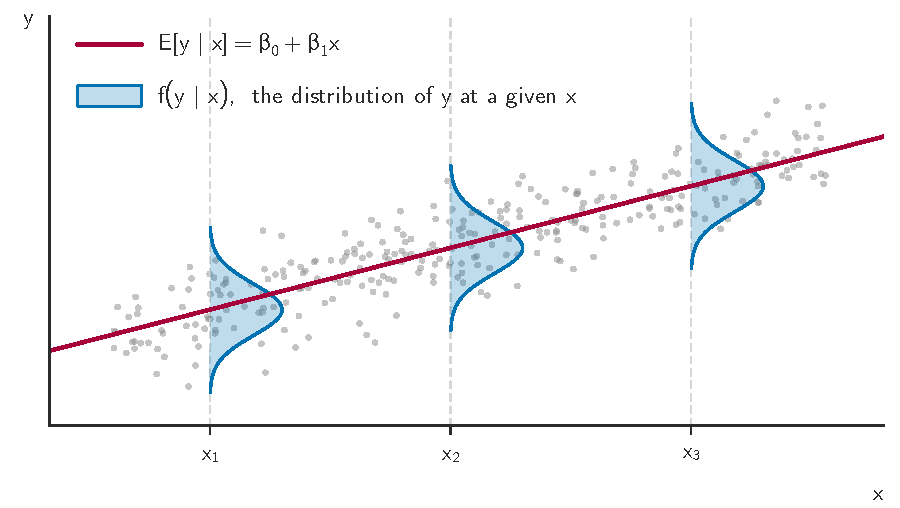
\includegraphics[height=0.82\textheight]{condvar_homo.pdf}
\end{figure}

}

\frame{
\frametitle{Example: $V[u_i|\X]=\sigma_i^2$ Heteroskedasticity}

\vspace{-.3cm}
\begin{figure}[ht] \centering
        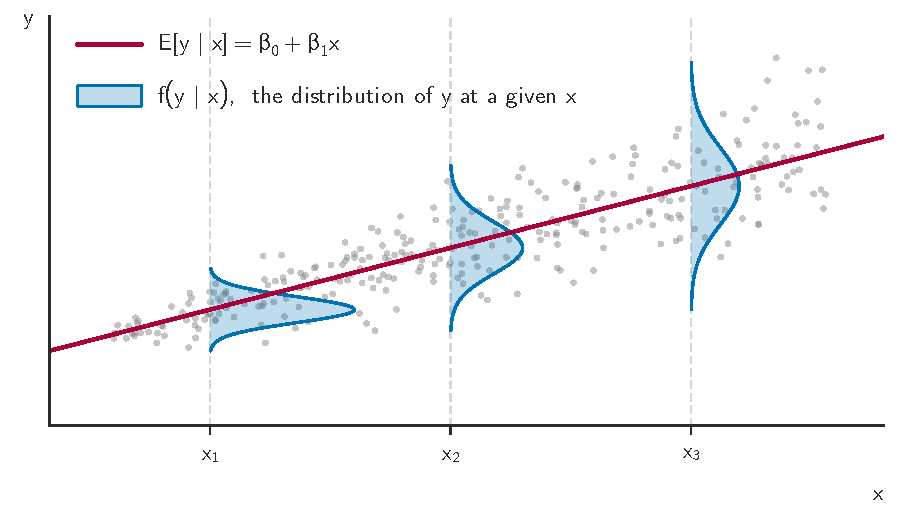
\includegraphics[height=0.82\textheight]{condvar_hetero.pdf}
\end{figure}

}

\frame{
\frametitle{Consequences of Heteroskedasticity}
\pause
\begin{itemize}
\item The usual estimator $\hat{\sigma}^2 \XXinv$ is no longer unbiased or consistent for $V[\hat{\b}|\X]$. This implies that the usual standard errors are no longer valid
\item Test statistics, which are functions of the standard errors, will no longer have $t$ and $F$ distributions.
\item For ``$\alpha$'' level tests, probability of Type I error will not be $\alpha$.
\item ``$1-\alpha$'' confidence intervals will not have $1-\alpha$ coverage probability.
  \item The OLS estimator is no longer BLUE.
\end{itemize}\pause\medskip

However,
\begin{itemize}
\item The degree of the problem depends on how serious the heteroskedasticity is.
\item If the other assumptions still hold (including zero conditional mean), $\bhat$ is still unbiased and consistent for $\b$. Why?
\end{itemize}

}

\frame{
\frametitle{Visual Diagnostics of Non-constant Error Variances}
Because we cannot directly observe the errors, we investigate \alert{residuals} to see if there is evidence for heteroskedasticity:
\bigskip
\begin{itemize}
  \item Under homoskedasticity, we expect the variance of the residuals to be constant across the fitted values and all the values of the explanatory variables \bigskip
\item We can therefore diagnose the plausibility of homoskedasticity by plotting:
	\begin{itemize}
	\item Residuals against fitted values ($\hat{y_i}$)
	\item Residuals against explanatory variables ($x_{ij}$)
	\end{itemize}
\end{itemize}
}


\frame{
\frametitle{Example: Buchanan Votes in Florida}

\begin{itemize}\itemsep1em
  \item We examine data from the 2000 presidential election in Florida used in Wand et al. (2001) \emph{APSR}.
  \item Our analysis takes place at the county level, and we will regress the number of Buchanan votes in each county on the total number of votes in each county.
  \item Nationwide Buchanan finished fourth in the presidential election with 0.4\% of the popular vote.
\end{itemize}
}

% \frame{
% \frametitle{Buchanan Votes and Total Votes}

% \vspace{-.3cm}
% \begin{figure}[ht] \centering
%         \scalebox{.45}{\includegraphics{fig1.pdf}}
% \end{figure}
% }

\frame{
\frametitle{Buchanan Votes and Total Votes}

\vspace{-.5cm}
\begin{figure}[ht] \centering
        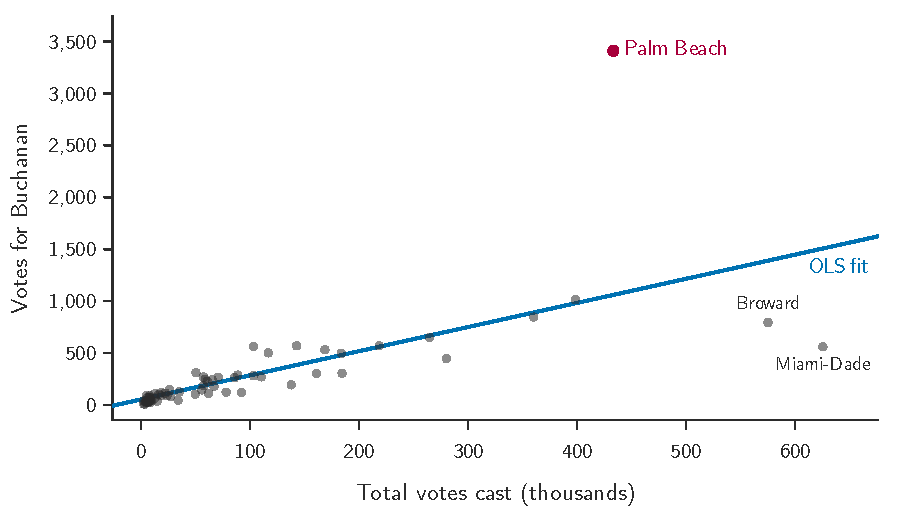
\includegraphics[height=0.82\textheight]{fl_votes.pdf}
\end{figure}

}

\frame{
\frametitle{The Butterfly Ballot}

\vspace{-.5cm}
\begin{figure}[ht] \centering
        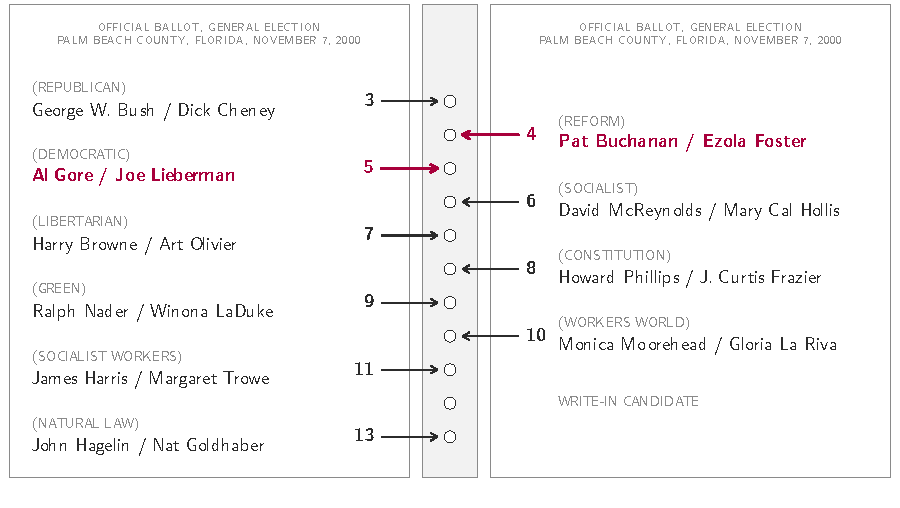
\includegraphics[height=0.58\textheight]{butterfly_ballot.pdf}
\end{figure}
\vspace{-.3cm}
Bush spokesman Ari Fleischer stated, ``Palm Beach county is a Pat Buchanan stronghold and that's why Pat Buchanan received 3,407 votes there.'' Buchanan said ``it's very easy for me to see how someone could have voted for me in the belief they voted for Al Gore''
}

\frame{
\frametitle{The Butterfly Ballot}

\vspace{-.5cm}
\begin{figure}[ht] \centering
        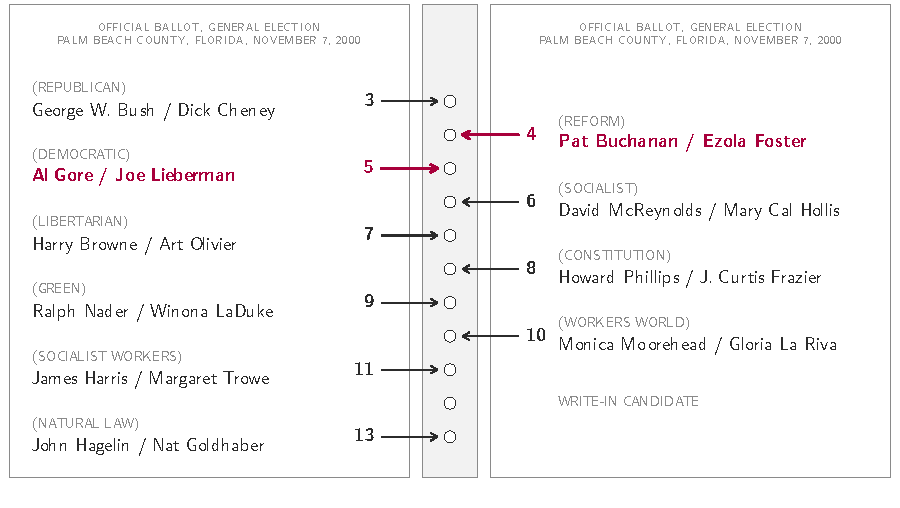
\includegraphics[height=0.58\textheight]{butterfly_ballot.pdf}
\end{figure}
\vspace{-.3cm}
Wand et al. (2001) conclude that the ballot caused more than 2,000 Democratic voters to vote by mistake for Buchanan, more than Bush's certified margin of 537 votes in Florida. Other things equal, Gore would have won Florida's 25 electoral votes and the presidency.
}


\begin{frame}[fragile]
\frametitle{Buchanan Votes and Total Votes}
\small

\begin{Verbatim}[fontsize=\scriptsize, frame=single, label=R Code, commandchars=\\\{\}]
> mod1 <- lm(buchanan00~TotalVotes00,data=dta)
> summary(mod1)
Residuals:
    Min      1Q  Median      3Q     Max
-947.05  -41.74  -19.47   20.20 2350.54

Coefficients:
              Estimate Std. Error t value Pr(>|t|)
(Intercept)  5.423e+01  4.914e+01   1.104    0.274
TotalVotes00 2.323e-03  3.104e-04   7.483 2.42e-10 ***
---
Residual standard error: 332.7 on 65 degrees of freedom
Multiple R-squared: 0.4628,	Adjusted R-squared: 0.4545
F-statistic:    56 on 1 and 65 DF,  p-value: 2.417e-10

> residuals              <- resid(mod1)
> standardized_residuals <- rstandard(mod1)
> studentized_residuals  <- rstudent(mod1)
> plot(fitted(mod1), residuals)
\end{Verbatim}
\end{frame}



\frame{
\frametitle{Example: Buchanan Votes in Florida -- Residuals}
\vspace{-.5cm}
\begin{figure}[ht] \centering
        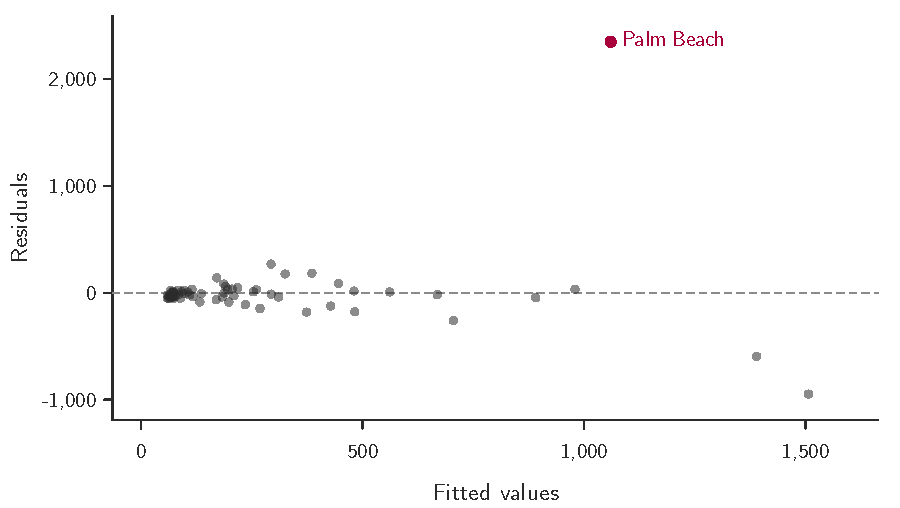
\includegraphics[height=0.82\textheight]{fl_resid.pdf}
\end{figure}
}


\frame{
\frametitle{Example: Buchanan Votes in Florida -- Magnitude of Residuals}
\small
\begin{columns} [c]
\begin{column}[]{7cm}
\begin{footnotesize}
\begin{itemize}
\uncover<1->{\item There is a positive relationship between total votes and votes for Buchanan.}
\uncover<2->{\item Plotting the residuals against the fitted values gives us some sense of the variance of the residuals}
\uncover<3->{\item We can do better by constructing the so-called \alert{spread-location plot}:} \medskip
\begin{itemize}\begin{footnotesize}

\uncover<4->{\item Standardize the residuals and take absolute values to fold the plot in half}
\uncover<5->{\item Add a smooth (loess) line to check if the variance varies with the fitted values}
\end{footnotesize}
\end{itemize}

\end{itemize}
\end{footnotesize}
\end{column}
\begin{column}[]{8cm}
\begin{overprint}
\onslide<1|handout:0>
\begin{figure}[ht] \centering
        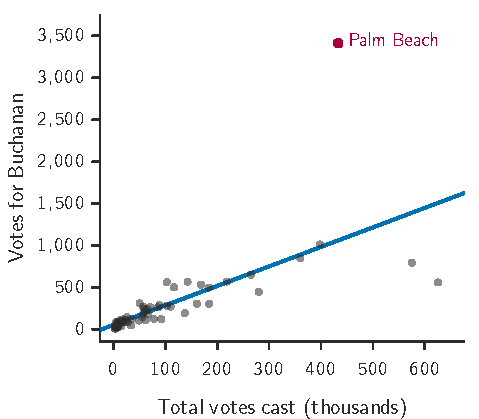
\includegraphics[width=0.889\linewidth]{fl_votes_col.pdf}
\end{figure}
\onslide<2-3|handout:0>
\begin{figure}[ht] \centering
        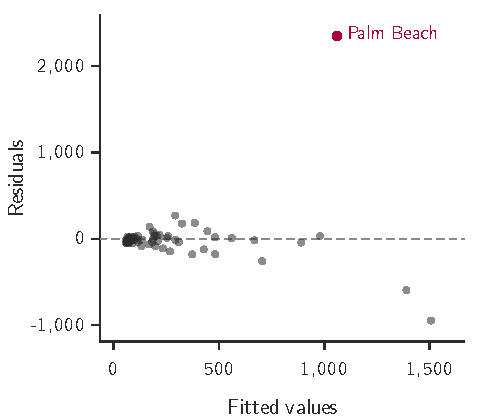
\includegraphics[width=0.889\linewidth]{fl_resid_col.pdf}
\end{figure}
\onslide<4|handout:0>
\begin{figure}[ht] \centering
        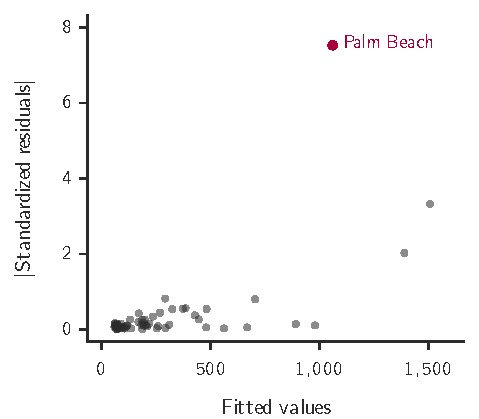
\includegraphics[width=0.889\linewidth]{fl_spread_col.pdf}
\end{figure}
\onslide<5|handout:1>
\begin{figure}[ht] \centering
        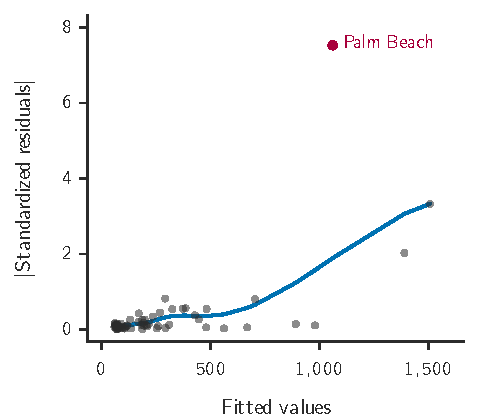
\includegraphics[width=0.889\linewidth]{fl_spread_loess_col.pdf}
\end{figure}
\end{overprint}

\end{column}
\end{columns}
}

\frame{
\frametitle{Buchanan Votes: Why the Spread Grows}
\begin{itemize}\itemsep1em
\item Buchanan votes is a \alert{count}, and the spread of a count grows with its size: for a pure count, roughly with the square root (ten times the voters, about three times the spread). So the spread of the residuals grows with county size.
\item The residual SD is 25 votes in the smallest third of counties, 60 in the middle third and 191 in the largest third (refit without Palm Beach).
\pause
\item Three big counties drive the fit in levels. Miami-Dade, Broward and Palm Beach cast 27\% of the votes. Their leverage $h_{ii}$ (the $i$th diagonal entry of the hat matrix $\mb{P}$) is .27, .22 and .12. The average is .03.
\item They pull the line in opposite directions. The slope is 2.32 Buchanan votes per 1,000 votes cast. It is 1.52 without Palm Beach and 3.67 without Miami-Dade and Broward.
\end{itemize}
}

\frame{
\frametitle{Formal Tests for Non-constant Error Variances}

\begin{itemize}
\addtolength{\itemsep}{.5\baselineskip}
  \item Plots are usually sufficient, but formal tests for heteroskedasticity exist (e.g. Breusch-Pagan, Cook-Weisberg, White, etc.).\\
\pause
      \item They are all roughly based on the same idea:
      \begin{itemize}
      \addtolength{\itemsep}{.5\baselineskip}
      \item $H_0$: $V[u_i|\X]= \sig$
      \item Under the zero conditional mean assumption, this is equivalent to \\
      $H_0$: $E[u_i^2|\X] = E[u_i^2] = \sig$, a constant unrelated to $\X$
      \item This implies that, under $H_0$, the \alert{squared residuals} should also be
      unrelated to the explanatory variables
      \end{itemize}
\pause
\item The \alert{Breusch-Pagan test}:
\begin{enumerate}
\addtolength{\itemsep}{.5\baselineskip}
\item Regress $y_i$ on $\x_i$ and store residuals $\hat{u}_i$
\item Regress $\hat{u_i}^2$ on $\x_i$
\item Test that all slope coefficients are zero (an $F$ test, or the $\chi^2$ statistic that {\tt bptest} reports)
\end{enumerate}
\pause
\begin{itemize}
\item In R, {\tt bptest} in the {\tt lmtest} package
\end{itemize}
\end{itemize}
}


\begin{frame}
\frametitle{Dealing with Non-constant Error Variances}
Once we detect a likely heteroskedasticity, how should we deal with it?
\medskip
\pause
\begin{enumerate}
  \addtolength{\itemsep}{.5\baselineskip}
  \item Use a \alert{variance stabilizing transformation} (this will affect the other model assumptions).
  \item Model the heteroskedasticity (e.g. \alert{Weighted Least Squares, WLS}). This needs a good ``weighting'' model. Not common in applied work. 
  \item Use an estimator of $V[\hat{\b}]$ that is \alert{robust to
  heteroskedasticity} (e.g. White's heteroskedasticity consistent estimator and its descendants).
  \item Admit that we have the wrong model and use an entirely different approach (e.g. nonlinear regression).
\end{enumerate}
\end{frame}

\begin{frame}
\frametitle{Variance Stabilizing Transformations}

Let $\sigma_i^2$ be the conditional variance of $Y_i$. If $\sigma_i^2$ is proportional to some function of the mean $\mu_i = \x_i \b$, then a variance stabilizing transformation may be appropriate.\\\bigskip

Note: Transformations will affect the other regression assumptions, as well as interpretation of the regression coefficients. \\
\begin{center}
\begin{tabular}{lc}
\hline
Transformation & Mean/Variance Relationship  \\
\hline
$\sqrt{Y}$ & $\sigma_i^2 \propto \mu_i$  \\
$\log Y$ & $\sigma_i^2 \propto \mu_i^2$   \\
$1/Y$ & $\sigma_i^2 \propto \mu_i^4$  \\
\hline
\end{tabular}
\end{center}
For example, if $\sigma_i^2 \propto \mu_i$, then by the Delta method,
\[
\operatorname{var}(\sqrt{Y_i} \mid \X)
\approx \tfrac{1}{4\mu_i}\operatorname{var}(Y_i \mid \X) = const.
\]
\end{frame}


\frame{
\frametitle{Example: Buchanan Votes in Florida}
\begin{columns} [c]
\begin{column}[]{7cm}
\begin{itemize}\itemsep1em
\uncover<1->{\item Things tend to look better after a log transformation of $Y$ and $X$}
\uncover<2->{\item We are much closer to a flat line now indicating that we approximately have a constant variance}
\uncover<3->{\item We could probably improve further by removing Palm Beach} \medskip
\end{itemize}
\end{column}
\begin{column}[]{9cm}
\begin{overprint}
\onslide<1|handout:0>
\begin{figure}[ht] \centering
        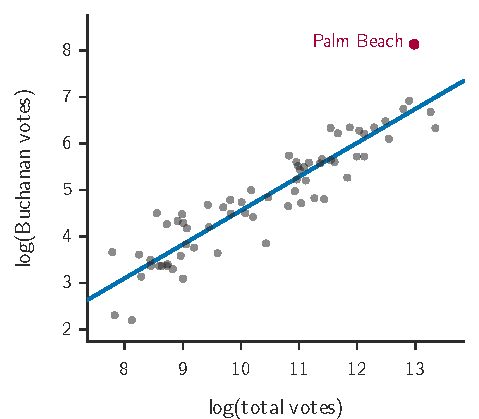
\includegraphics[width=0.79\linewidth]{fl_log_votes_col.pdf}
\end{figure}
\onslide<2|handout:0>
\begin{figure}[ht] \centering
        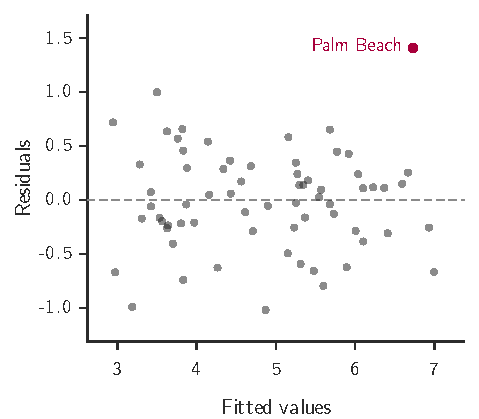
\includegraphics[width=0.79\linewidth]{fl_log_resid_col.pdf}
\end{figure}
\onslide<3|handout:1>
\begin{figure}[ht] \centering
        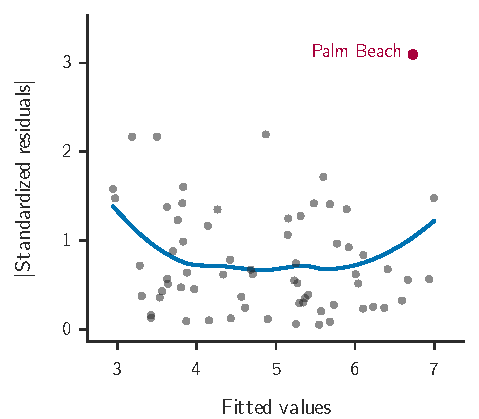
\includegraphics[width=0.79\linewidth]{fl_log_spread_loess_col.pdf}
\end{figure}
\end{overprint}
\end{column}
\end{columns}
}


\begin{frame}[fragile]
\frametitle{Example: Buchanan Votes in Florida}
The Breusch-Pagan test rejects constant variance in levels but not in logs (not rejecting does not prove constant variance):

\medskip
\begin{Verbatim}[fontsize=\scriptsize, frame=single, label=R Code, commandchars=\\\{\}]
> library(lmtest)
> mod1 <- lm(buchanan00 ~ TotalVotes00, data=dta)
> bptest(mod1, studentize = FALSE)

	Breusch-Pagan test

data:  mod1
BP = 250.0671, df = 1, p-value < 2.2e-16
> dta$lnbuchanan00 <- log(dta$buchanan00)
> dta$lnTotalVotes00 <- log(dta$TotalVotes00)
> mod2 <- lm(lnbuchanan00 ~ lnTotalVotes00, data=dta)
> bptest(mod2, studentize = FALSE)

	Breusch-Pagan test

data:  mod2
BP = 0.0111, df = 1, p-value = 0.916
\end{Verbatim}
{\footnotesize With {\tt bptest}'s default (Koenker's studentized version): BP = 12.6, $p = 0.0004$ in levels; BP = 0.010, $p = 0.92$ in logs.}

\end{frame}


%\frame{
%
%\frametitle{Weighted Least Squares}
%\small
%\vspace{-.5\baselineskip}
%\begin{itemize}
% \item If we have a good model of the heteroskedasticity, we can use \alert{weighted least squares (WLS)} to obtain a BLUE estimator.
% \pause
% \item Suppose that the heteroskedasticity is known up to a multiplicative constant:
% $$ V[u_i \mid \X] = a_i \sig $$
% where $a_i = a_i(\x_i)$ is a positive and known function of $\x_i$.
% \pause
% \item In this setting, we can obtain a BLUE estimator of $\b$ by multiplying the regression equation by \alert{$1/\sqrt{a_i}$}:
% $$ y_i\alert{/\sqrt{a_i}} \ = \ \beta_0\alert{/\sqrt{a_i}} + \beta_1 x_{i1}\alert{/\sqrt{a_i}} + \cdots + \beta_k x_{ik}\alert{/\sqrt{a_i}} + u_i\alert{/\sqrt{a_i}} $$
% \pause
% or, using the matrix notation,
% $$ \mb{W} \y \ = \ \mb{W} \X \b + \mb{W} \u $$
% where
%$$
%\mb{W} =\left[
%                                                 \begin{array}{cccc}
%                                                   1/\sqrt{a_1}  & 0 & 0 & 0 \\
%                                                   0 & 1/\sqrt{a_2}  & 0 & 0 \\
%                                                   \vdots & \vdots & \ddots & \vdots \\
%                                                   0 & 0 & 0 & 1/\sqrt{a_n}  \\
%                                                 \end{array}
%                                               \right]
%                                               $$
%\end{itemize}
%}
%
%\begin{frame}
%\frametitle{Why Does WLS Work?}
%\small
%If the untransformed regression model satisfies the OLS assumptions other than homoskedasticity, then the transformed regression satisfies all the OLS assumptions, and is therefore BLUE.
%\pause
%\begin{itemize}
%    \item For example, the zero conditional mean assumption is maintained after the transformation:
%    $$ E\l[\frac{u_i}{\sqrt{a_i}}\mid \x_i\r] = \frac{1}{\sqrt{a_i}}E\l[u_i\mid \x_i\r] = 0$$
%    so the transformed regression remains unbiased and consistent.
%    \medskip
%    \pause
%    \item The transformed regression also has a homoskedastic error:
%    $$ V\l[\frac{u_i}{\sqrt{a_i}}|\x_i\r] = E\l[\l(\frac{u_i}{\sqrt{a_i}}\r)^2 |\x_i\r] =
%    \frac{E[u_i^2 \mid \x_i]}{a_i} = \frac{\sigma^2 a_i}{a_i} = \sigma^2$$
%\end{itemize}
%\pause
%Note that this requires that we know the correct form of heteroskedasticity, which
%is rarely the case in practice.
%
%\end{frame}
%
%
%\frame{
%\frametitle{WLS Estimating Procedures}
%\small
%\vspace{-.5\baselineskip}
%\begin{itemize}
%  \item Two step estimation:
% \begin{enumerate}
%  \item  Transform the data by dividing each variable by $\sqrt{a_i}$
%  \item Run OLS in the transformed data
%  \end{enumerate}
%\pause
%\item One step estimation: Create the weight matrix $\mb{V} = \mb{W}\mb{W}$, i.e.,
%$$
%\mb{V} =\left[
%                                                 \begin{array}{cccc}
%                                                   1/a_1  & 0 & 0 & 0 \\
%                                                   0 & 1/a_2  & 0 & 0 \\
%                                                   \vdots & \vdots & \ddots & \vdots \\
%                                                   0 & 0 & 0 & 1/a_n  \\
%                                                 \end{array}
%                                               \right]
%$$
%and the WLS estimator for $\b$ is given by:
%$$
%\hat\b_W \ = \ (\X' \mb{V}\X)^{-1}\X' \mb{V} \y
%$$
%\vspace{-\baselineskip}
%\pause
%\item The one-step estimator can be derived by minimizing the weighted SSR:
%$$
%\hat\b_W \ = \ \argmin_{\b} \sum_{i=1}^n \l(\frac{\hat{u}_i}{\sqrt{a_i}}\r)^2
% \ = \ \argmin_{\b} \ \u'\mb{V}\u
%$$
%  \item Note that OLS can be thought of as a special case where we assume $\mb{V} = \mb{I}$
%\end{itemize}
%
%}
%
%
%\begin{frame}[fragile]
%\frametitle{Example: Buchanan Votes in Florida}
%\small
%To fit WLS in R, we can use the {\tt lm} command with the {\tt weights} argument:
%\medskip
%\begin{Verbatim}[fontsize=\scriptsize, frame=single, label=R Code, commandchars=\\\{\}]
%> modwls <- lm(buchanan00 ~ TotalVotes00, \alert{weights=1/TotalVotes00}, data=dta)
%> summary(modwls)
%
%Call:
%lm(formula = buchanan00 ~ TotalVotes00, data = dta, weights = 1/TotalVotes00)
%
%Weighted Residuals:
%    Min      1Q  Median      3Q     Max
%-1.4046 -0.2146 -0.0501  0.1971  3.4117
%
%Coefficients:
%              Estimate Std. Error t value Pr(>|t|)
%(Intercept)  2.707e+01  8.507e+00   3.182  0.00224 **
%TotalVotes00 2.628e-03  2.502e-04  10.503 1.22e-15 ***
%---
%Signif. codes:  0 '***' 0.001 '**' 0.01 '*' 0.05 '.' 0.1 ' ' 1
%
%Residual standard error: 0.5646 on 65 degrees of freedom
%Multiple R-squared: 0.6292,	Adjusted R-squared: 0.6235
%F-statistic: 110.3 on 1 and 65 DF,  p-value: 1.221e-15
%\end{Verbatim}
%\end{frame}
%
%
%\begin{frame}
%\frametitle{Example: Buchanan Votes in Florida}
%\small
%In the Florida example, although it seems reasonable to assume that the error
%variance increases with the total votes, WLS appears to help only slightly:
%\begin{center}
%\includegraphics[width=\textwidth]{Buchanan-OLSWLS.pdf}
%\end{center}
%
%\end{frame}



\frame{
\frametitle{White's Heteroskedasticity Consistent Estimator}

Let's go back to our derivation of the variance of the regression estimator, when the error structure, $\alert{\bs{\Sigma}}$, may be heteroskedastic:
\begin{align*}
V[\hat{\b}|\X] &= V[\b|\X] + V[\XXinv \X' \mb{u}|\X] \\
                   &= V[ \XXinv \X'  \mb{u}|\X]  \\
                    &=  \XXinv \X'  \alert{V[\mb{u}|\X]}  (\XXinv \X')' \,\,(\mbox{note: $\X$ nonrandom $|\X$})   \\
                 &=  \XXinv \X'  \alert{V[\mb{u}|\X]}  \X \XXinv   \\
                   &=  \XXinv \X'  \alert{\bs{\Sigma} }  \X \XXinv
\end{align*}\\\medskip
Idea: one squared residual cannot estimate each $\sigma_i^2$ well, but we only need the $(k+1)\times(k+1)$ average $\frac{1}{n}\X'\bs{\Sigma}\X$, and $\frac{1}{n}\X'\bs{\hat{\Sigma}}\X$ estimates it consistently.
}


\begin{frame}[fragile]
\frametitle{White's Heteroskedasticity Consistent Estimator}
\begin{small}
Suppose we have \alert{heteroskedasticity of unknown form}:
$$
V[\u] = \alert{\bs{\Sigma}} =  \left[ \begin{array}{ccccc} \sigma_1^2 & 0 & 0 & \dots & 0 \\
0 & \sigma_2^2 & 0 & \dots & 0 \\
 & & & \vdots & \\
 0 & 0 & 0 & \dots & \sigma_n^2 \end{array} \right]
$$
\pause
then $V[\hat{\b}|\X] = \XXinv \X' \alert{\bs{\Sigma}} \X \XXinv$ and White (1980) shows that
\pause
$$\widehat{V[\hat{\b}|\X]}=
\XXinv \X' \left[ \begin{array}{ccccc} \hat{\u}_1^2 & 0 & 0 & \dots & 0 \\
0 & \hat{\u}_2^2 & 0 & \dots & 0 \\
 & & & \vdots & \\
 0 & 0 & 0 & \dots & \hat{\u}_n^2 \end{array} \right] \X \XXinv
$$
is a consistent estimator of $V[\hat{\b}|\X]$  \alert{under any form of heteroskedasticity}, as long as the observations are independent. \\
\medskip

The estimate based on the above is called the \alert{heteroskedasticity consistent (HC)} or
\alert{robust standard errors}.
\end{small}
\end{frame}

\begin{frame}[fragile]
\frametitle{White's Heteroskedasticity Consistent Estimator}
\begin{small}
Robust standard errors are easily computed with the ``sandwich'' formula:

\begin{enumerate}
  \item Fit the regression and obtain the residuals $\hat{\mb{u}}$
  \item Construct $\widehat{\bs{\Sigma}}$ with the squared residuals on the diagonal (the ``meat'' of the sandwich is $\X'\widehat{\bs{\Sigma}}\X$; the ``bread'' is $\XXinv$):
  $$\widehat{\bs{\Sigma}}=
 \left[ \begin{array}{ccccc} \hat{\u}_1^2 & 0 & 0 & \dots & 0 \\
0 & \hat{\u}_2^2 & 0 & \dots & 0 \\
 & & & \vdots & \\
 0 & 0 & 0 & \dots & \hat{\u}_n^2 \end{array} \right]
$$
\item Plug $\widehat{\bs{\Sigma}}$ into the sandwich formula to obtain the robust estimator of the variance-covariance matrix$$
\widehat{V}_{HC0}[\hat{\b}|\X] = \XXinv \X' \widehat{\bs{\Sigma}} \X \XXinv
$$
\end{enumerate}
\end{small}
\pause
\footnotesize{
\begin{itemize}
\item There are various \alert{small sample corrections} to improve performance when sample size is small. The most common variant (sometimes labeled HC1) is:
$$ \widehat{V}_{HC1}[\hat{\b}|\X] \ = \ \frac{n}{n-k-1} \cdot \XXinv \X' \widehat{\bs{\Sigma}} \X \XXinv $$
\end{itemize}
}
\end{frame}



\begin{frame}[fragile]
\frametitle{Regular \& Robust Standard Errors in Florida Example}

\begin{Verbatim}[fontsize=\scriptsize, frame=single, label=R Code, commandchars=\\\{\}]
> library(sandwich)
> library(lmtest)
> coeftest(mod1) \alert{# homoskedasticity}
t test of coefficients:
               Estimate Std. Error t value  Pr(>|t|)
(Intercept)  5.4231e+01 4.9141e+01  1.1036    0.2738
TotalVotes00 2.3229e-03 3.1041e-04  7.4831 2.417e-10 ***

> coeftest(mod1,vcov = vcovHC(mod1, type = "HC0")) \alert{# classic White}
t test of coefficients:
               Estimate Std. Error t value Pr(>|t|)
(Intercept)  5.4231e+01 4.0612e+01  1.3353  0.18642
TotalVotes00 2.3229e-03 8.7047e-04  2.6685  0.00961 **

> coeftest(mod1,vcov = vcovHC(mod1, type = "HC1")) \alert{# small sample correction}
t test of coefficients:
               Estimate Std. Error t value Pr(>|t|)
(Intercept)  5.4231e+01 4.1232e+01  1.3153  0.19304
TotalVotes00 2.3229e-03 8.8376e-04  2.6284  0.01069 *
\end{Verbatim}
\end{frame}

\frame{
\frametitle{Florida: HC3, and Without Palm Beach}
\small
\begin{itemize}
\item \alert{HC3} puts $\hat u_i^2/(1-h_{ii})^2$ on the diagonal of $\widehat{\bs{\Sigma}}$ instead of $\hat u_i^2$.
\item This matters with high-leverage points. OLS pulls the line toward them, so their residuals understate their errors. HC3 scales these residuals back up. Miami-Dade's squared residual counts 1.85 times.
\end{itemize}
\medskip
\begin{center}
\begin{tabular}{lcc}
\hline
Slope and SEs (per 1,000 votes cast) & All 67 counties & Without Palm Beach \\
\hline
Slope & 2.32 & 1.52 \\
Classical SE & 0.31 & 0.12 \\
HC0 & 0.87 & 0.29 \\
HC1 & 0.88 & 0.30 \\
HC3 & 1.05 & 0.40 \\
\hline
\end{tabular}
\end{center}
\medskip
\pause
\begin{itemize}
\item The unequal spread is not only Palm Beach. Without it, the Breusch-Pagan test still rejects ($p < .001$), and the robust SE (HC1) is 2.5 times the classical SE.
\end{itemize}
}


% \frame{
% \frametitle{%WLS vs.
% White's Estimator}
% %WLS
% %\begin{itemize}
% %\item If the weights $a_1, ... , a_n$ are known, the WLS estimator for $\b$ is efficient,
% %\item and $\widehat{SE}[\hat{\b}_{WLS}]$ is unbiased and consistent.
% %\item The weights are usually not known.
% %\end{itemize}
% %\vspace{.5cm}
% %\pause
% }


\frame{
\frametitle{White's Estimator}
White's estimator: $$\widehat V_{HC0} \equiv \widehat{V}[\hat{\b}|\X] = (\X'\X)^{-1}\X'\bs{\widehat\Sigma}\X(\X'\X)^{-1}$$
\begin{itemize}\itemsep1em
\item White's estimator does not change our point estimate $\hat{\b}$
\item White's estimator for $V[\hat{\b}]$ is consistent for any form of heteroskedasticity.
\item If $n$ is large, you can get approximately correct CI coverage and test levels.
\item For small $n$, sometimes a correction factor is utilized to improve performance, but this is often insufficient to address the problem.
\end{itemize}
}

\frame{
\frametitle{White's Estimator}
\textbf{Worksheet Q1} The classic variance estimator is
\[
\widehat V_{0}
= \hat\sigma^2(\X'\X)^{-1}.
\]
The White estimator is
\[
\widehat V_{HC0}
= (\X'\X)^{-1}\X'\mathrm{diag}(\hat u_1^2,\ldots,\hat u_n^2)\X(\X'\X)^{-1}.
\]
Assume (1) $E[u_i\mid \X]=0$; (2) $\var(u_i\mid\X)=\sigma^2$; (3) $\frac{1}{n}\X'\X\to Q\succ0$; and (4) standard regularity conditions. Show that
\[
\plim (n\,\widehat V_0)=\plim (n\,\widehat V_{HC0})=\sigma^2 Q^{-1}.
\]

\noindent\textbf{Hint:}
\[
\frac{1}{n}\sum_{i=1}^n \x_i\x_i'\hat u_i^2
= \frac{1}{n}\sum_{i=1}^n \x_i\x_i' u_i^2 + o_p(1)
\xrightarrow{p}\sigma^2 E[\x_i\x_i']=\sigma^2 Q.
\]


}




\section{Clustering}

%\section{Some Common Types of Dependence}
%
%\frame{
%\frametitle{Variance of $\hat{\b}$}
%
%\begin{align*}
%\hat{\b} &= \XXinv \X' \y \\
%&=  \XXinv \X' (\X\b + \u) \\
%&= \b + \XXinv \X' \u
%\end{align*}
%
%\begin{align*}
%V[\hat{\b}] &= V[ \XXinv \X' \u] \\
%&= \XXinv \X'E[\u \u'] \X \XXinv \\
%&= \XXinv \X' \alert{\Sig} \X \XXinv
%\end{align*}
%
%}

%\frame{
%\frametitle{Constant Error Variance and Dependence}
%
%Assuming that the mean function is $\X\b$ and normality holds:
%
%$$
%\u \sim N_n(0,\Sig)
%$$
%
%where in general
%
%$$
%\Sig = Var(\u) = E[\u\u'] \alert{\ne} \left[ \begin{array}{ccccc} \sigma^2 & 0 & 0 & \dots & 0 \\
%0 & \sigma^2 & 0 & \dots & 0 \\
% & & & \vdots & \\
% 0 & 0 & 0 & \dots & \sigma^2 \end{array} \right]
%$$
%
%}
%
%\frame{
%\frametitle{Generalized Least Squares}
%
%\begin{align*}
%\hat{\b}^{GLS} &= (\X' \SigInv \X)^{-1} \X' \SigInv \y \\
%E[\hat{\b}^{GLS}] &=  (\X' \SigInv \X)^{-1} \X' \SigInv \X \b \\
%&=  \b
%\end{align*}
%
%\begin{align*}
%V[\hat{\b}^{GLS}] &= V[ (\X' \SigInv \X)^{-1} \X' \SigInv  \u] \\
%&= (\X' \SigInv \X)^{-1}
%\end{align*}
%
%$\hat{\b}^{GLS}$ is  BLUE.
%}


\frame{
\frametitle{Cluster Dependence: Intuition}
\small
\pause
\begin{itemize}
  \item Assume we draw a random sample of households and randomly assign half of them to an encouragement to vote
  \item We measure turnout for all individuals and regress this outcome on a treatment indicator
  \item How does this violate our regression assumptions? \pause
  \begin{itemize}
  \addtolength{\itemsep}{.25\baselineskip}
  \item Regression assumes that individuals are sampled independently, but this is not true because sampling and the intervention occurred at the household level, not at the level of individuals
 \item Errors/outcomes of individuals in the same household are correlated so by assuming independence we overstate the amount of information
    \item Because the treatment is the same for everyone in a household and the errors are positively correlated within households, conventional standard errors will be biased downward
  \end{itemize}
   \item Scenario is called \alert{clustering} or \alert{cluster dependence} and this problem is very common in many social science data applications.
\end{itemize}
}

\frame{
\frametitle{Cluster Dependence: Intuition}
\begin{itemize}
\item Often in social research \alert{units $i=1,...,N$} are nested within \textcolor{blue}{clusters $j=1,...,M$}
\item Clusters could be any grouping that could be expected to lead to dependencies:
\begin{itemize}
  \item \alert{voters} in \textcolor{blue}{households}
  \item \alert{individuals} in \textcolor{blue}{states}
  \item \alert{students} in \textcolor{blue}{classes}
  \item \alert{rulings} by \textcolor{blue}{judges}
  \item \alert{yearly inflation rates} of \textcolor{blue}{countries}
\end{itemize}
 \item Two types of clustering: clustering in sampling and clustering in assignment
  \item ``Randomization by cluster accompanied by an analysis appropriate to randomization by individual is an exercise in self-deception'' (Cornfield 1978, pp. 101--102)
  \item ``making a data set larger by copying a smaller one $n$ times generates no
new information'' (Angrist and Pischke 2009)
\end{itemize}
}




\frame{
\frametitle{Cluster Dependence: A Formal Definition}
\small
Assume \alert{units $i=1,...,N$} are nested within \textcolor{blue}{clusters $j=1,...,M$} (e.g. voters within households, students within classes, etc.).\\\bigskip
\pause
We assume a variance structure that allows the errors to be:
\begin{itemize}
  \item potentially correlated for units within the same cluster (correlation within)
  \item uncorrelated for units across clusters (independence across)
\end{itemize}\bigskip\pause
Our model with cluster dependence is:
$$
y_{ij} \ = \ \beta_0 + \beta_1 x_{ij} + {\mb \varepsilon}_{ij} \ = \
\beta_0 + \beta_1 x_{ij} + \textcolor{blue}{v_j} + \alert{u_{ij}},
$$
where
\begin{itemize}
  \item \textcolor{blue}{$v_j \iid N(0, \rho\sigma^2)$} cluster error component \pause
  \item \alert{$u_{ij} \iid N(0, (1-\rho)\sigma^2)$} unit error component \pause
  \item Note that $v_j$ and $u_{ij}$ are assumed to be independent of each other and $x_{i,j}$ \pause
  \item $\rho$ is called the \alert{within-cluster correlation}
\end{itemize}
}





\frame{
\frametitle{Cluster Dependence: Example}
\small
\textbf{Worksheet Q2}\\
Suppose we have $M=2$ clusters and $N=6$ units:
cluster $1$ contains units $i=1,2,3$ and cluster $2$ contains units $i=4,5,6$.
Stack the errors in the order
\[
\bm{\varepsilon}
=
(\varepsilon_{1,1},\varepsilon_{2,1},\varepsilon_{3,1},
\varepsilon_{4,2},\varepsilon_{5,2},\varepsilon_{6,2})'.
\]

\begin{enumerate}
\item Show that $V[\varepsilon_{ij}] = \sigma^2$ for all $i,j$.

\item For two units $i\neq \ell$ in the \emph{same} cluster $j$, compute $\cov(\varepsilon_{ij},\varepsilon_{\ell j}).$

\item For units in \emph{different} clusters $j\neq k$, compute $\cov(\varepsilon_{ij},\varepsilon_{\ell k}).$

\item Using your answers above, write out the $6\times 6$ covariance matrix $\Sigma = V[\bm{\varepsilon}]$ for the given ordering
$(\varepsilon_{1,1},\varepsilon_{2,1},\varepsilon_{3,1},
\varepsilon_{4,2},\varepsilon_{5,2},\varepsilon_{6,2})'$.

\item Compute the correlation $\cor(\varepsilon_{ij},\varepsilon_{\ell j})$
for $i\neq \ell$ in the same cluster $j$ and verify that it equals $\rho$.
\end{enumerate}
}

\frame{
\frametitle{Cluster Dependence: Example}
\footnotesize
$\bm{\varepsilon}=\left[
\begin{array}{cccccc}
  \textcolor{orange}{\varepsilon_{1,1}} & \textcolor{orange}{\varepsilon_{2,1}} & \textcolor{orange}{\varepsilon_{3,1}} & \textcolor{green}{\varepsilon_{4,2}} & \textcolor{green}{\varepsilon_{5,2}} & \textcolor{green}{\varepsilon_{6,2}}  \end{array}\right]'$\\\bigskip
  $V[\bm{\varepsilon}]=\Sig=$
 \pause
$\left[
\begin{array}{cccccc}
 V[\textcolor{orange}{\varepsilon_{1,1}}]  & Cov[\textcolor{orange}{\varepsilon_{2,1}},\textcolor{orange}{\varepsilon_{1,1}}]  &  Cov[\textcolor{orange}{\varepsilon_{3,1}},\textcolor{orange}{\varepsilon_{1,1}}]  & . &. & . \\
  Cov[\textcolor{orange}{\varepsilon_{1,1}},\textcolor{orange}{\varepsilon_{2,1}}]  & V[\textcolor{orange}{\varepsilon_{2,1}}] &  Cov[\textcolor{orange}{\varepsilon_{3,1}},\textcolor{orange}{\varepsilon_{2,1}}]  & . & . & . \\
 Cov[\textcolor{orange}{\varepsilon_{1,1}},\textcolor{orange}{\varepsilon_{3,1}}]  & Cov[\textcolor{orange}{\varepsilon_{2,1}},\textcolor{orange}{\varepsilon_{3,1}}]  & V[\textcolor{orange}{\varepsilon_{3,1}}] & . & . & . \\
Cov[\textcolor{orange}{\varepsilon_{1,1}},\textcolor{green}{\varepsilon_{4,2}}]   & Cov[\textcolor{orange}{\varepsilon_{2,1}},\textcolor{green}{\varepsilon_{4,2}}] & Cov[\textcolor{orange}{\varepsilon_{3,1}},\textcolor{green}{\varepsilon_{4,2}}] & V[\textcolor{green}{\varepsilon_{4,2}}] & .  &  .\\
Cov[\textcolor{orange}{\varepsilon_{1,1}},\textcolor{green}{\varepsilon_{5,2}}]    & Cov[\textcolor{orange}{\varepsilon_{2,1}},\textcolor{green}{\varepsilon_{5,2}}]  & Cov[\textcolor{orange}{\varepsilon_{3,1}},\textcolor{green}{\varepsilon_{5,2}}]  & Cov[\textcolor{green}{\varepsilon_{4,2}},\textcolor{green}{\varepsilon_{5,2}}] & V[\textcolor{green}{\varepsilon_{5,2}}] & . \\
 Cov[\textcolor{orange}{\varepsilon_{1,1}},\textcolor{green}{\varepsilon_{6,2}}]  & Cov[\textcolor{orange}{\varepsilon_{2,1}},\textcolor{green}{\varepsilon_{6,2}}] & Cov[\textcolor{orange}{\varepsilon_{3,1}},\textcolor{green}{\varepsilon_{6,2}}] & Cov[\textcolor{green}{\varepsilon_{4,2}},\textcolor{green}{\varepsilon_{6,2}}] & Cov[\textcolor{green}{\varepsilon_{5,2}},\textcolor{green}{\varepsilon_{6,2}}]  & V[\textcolor{green}{\varepsilon_{6,2}}]
\end{array}\right]$\\\bigskip\pause
$=$
$\left[\begin{array}{cccccc}
 \sigma^2  & \sigma^2 \cdot \rho  &  \sigma^2 \cdot \rho  & 0 & 0 & 0 \\
  \sigma^2 \cdot \rho  & \sigma^2 &  \sigma^2 \cdot \rho  & 0 & 0 & 0 \\
 \sigma^2 \cdot \rho  & \sigma^2 \cdot \rho  & \sigma^2 & 0 & 0 & 0 \\
0  & 0 & 0 & \sigma^2 & \sigma^2 \cdot \rho  &  \sigma^2 \cdot \rho\\
0   & 0 & 0  & \sigma^2 \cdot \rho & \sigma^2 & \sigma^2 \cdot \rho \\
0  & 0 & 0 & \sigma^2 \cdot \rho & \sigma^2 \cdot \rho  & \sigma^2
\end{array}\right]
$
%\\\bigskip
% which can be verified as follows:
% \begin{itemize}
% \addtolength{\itemsep}{.15\baselineskip}
% \item
% $V[\textcolor{orange}{\varepsilon_{ij}}]=\pause V[\textcolor{blue}{v_j} +\alert{u_{ij}}]=V[\textcolor{blue}{v_j}] +V[\alert{u_{ij}}]=\rho \sigma^2 + (1-\rho) \sigma^2=\sigma^2$ \pause
% \item
% $Cov[\textcolor{orange}{\varepsilon_{ij}},\textcolor{orange}{\varepsilon_{lj}}] = E[(\textcolor{blue}{v_j} +\alert{u_{ij}})(\textcolor{blue}{v_j} +\alert{u_{lj}})] $\\
% \pause $ =  E[\textcolor{blue}{v_j}^2]+E[\textcolor{blue}{v_j}\alert{u_{ij}}] + E[\textcolor{blue}{v_j}\alert{u_{lj}}] + E[\alert{u_{ij}}\alert{u_{lj}}] $ \\
% \pause $ =  E[\textcolor{blue}{v_j}^2]+E[\textcolor{blue}{v_j}]E[\alert{u_{ij}}] + E[\textcolor{blue}{v_j}]E[\alert{u_{lj}}] + E[\alert{u_{ij}}]E[\alert{u_{lj}}] $ \\
% $ = E[\textcolor{blue}{v_j}^2] =  V[\textcolor{blue}{v_j}] + (E[\textcolor{blue}{v_j}])^2  =  V[\textcolor{blue}{v_j}]  = \rho \sigma^2$ \pause
% \item
% $Cov[\textcolor{orange}{\varepsilon_{ij}},\textcolor{green}{\varepsilon_{lk}}]
% = E[(\textcolor{blue}{v_j} +\alert{u_{ij}})(\textcolor{blue}{v_k} +\alert{u_{lk}})] $ \\
% $ = E[\textcolor{blue}{v_j} \textcolor{blue}{v_k}]+E[\textcolor{blue}{v_j}\alert{u_{lk}}]  +  E[\textcolor{blue}{v_k}\alert{u_{ij}}]  +E[\alert{u_{ij}}\alert{u_{lk}}]  $\\
% $ = E[\textcolor{blue}{v_j}]E[ \textcolor{blue}{v_k}]+E[\textcolor{blue}{v_j}]E[\alert{u_{lk}}]  +  E[\textcolor{blue}{v_k}]E[\alert{u_{ij}}]  +E[\alert{u_{ij}}]E[\alert{u_{lk}}]
% =0$
% \end{itemize}
}


\frame{
\frametitle{Error Variance Matrix with Cluster Dependence}
\small
The variance-covariance matrix of the error, $\Sig$, is \alert{block diagonal}:
\begin{itemize}
\item By independence, the errors are uncorrelated across clusters:$$
V[\bm{\varepsilon}] = \Sig  = \left[ \begin{array}{c|c|c|c} \Sig_1 & 0 & \dots & 0 \\
\hline
\mb{0} & \Sig_2 &  \dots & \mb{0} \\
 \hline
 & &  \ddots & \\
 \hline
 \mb{0} & \mb{0} & \dots & \Sig_M \end{array} \right]
$$
\item But the errors may be correlated for units within the same cluster:\pause
$$
\Sig_j = \left[ \begin{array}{cccc} \sigma^2   & \sigma^2 \cdot \rho &  \dots & \sigma^2 \cdot \rho \\
\sigma^2 \cdot \rho & \sigma^2 &  \dots & \sigma^2 \cdot \rho \\
 & &  \ddots & \\
 \sigma^2 \cdot \rho & \sigma^2 \cdot \rho & \dots & \sigma^2 \end{array} \right]
$$
\end{itemize}
}

% \frame{
% \frametitle{Estimating the Variance Components: $\rho$ and $\sigma^2$ }
% \small
% The overall error variance $\sigma^2$ is easily estimated using our usual estimator based on the regression residuals: $\widehat{\sigma}^2=\frac{\hat{\bm{\varepsilon}}'\hat{\bm{\varepsilon}}}{N-k-1}$\\\bigskip\pause

% The within-cluster correlation can be estimated as follows:
% \begin{enumerate}
%   \item Subtract from each residual $\hat{\varepsilon}_{ij}$ the mean residual within its cluster. Call this vector of demeaned residuals $\tilde{\bm{\varepsilon}}$, which estimates the
%   unit error component $\bm{u}$ \pause\medskip
%   \item Compute the variance of the demeaned residuals as: $\widehat{\tilde{\sigma}}^2=\frac{\tilde{\bm{\varepsilon}}'\tilde{\bm{\varepsilon}}}{N-M-k-1}$, which estimates $(1-\rho)\sigma^2$ \pause\medskip
%   \item The within cluster correlation is then estimated as: $\hat{\rho}=\frac{\widehat{\sigma}^2 - \widehat{\tilde{\sigma}}^2}{\widehat{\sigma}^2}$
% \end{enumerate}

% }


% \begin{frame}[fragile]
% \frametitle{Estimating Cluster Robust Standard Errors}
% {\footnotesize
% \begin{enumerate}
%   \item Take your estimates of $\widehat{\sigma^2}$ and $\widehat{\rho}$ and construct the block diagonal variance-covariance matrix $\widehat{\Sig}$:
% $$
% \widehat{\Sig}  = \left[ \begin{array}{c|c|c|c} \widehat{\Sig_1} & 0 & \dots & 0 \\
% \hline
% \mb{0} & \widehat{\Sig_2} &  \dots & \mb{0} \\
%  \hline
%  & &  \ddots & \\
%  \hline
%  \mb{0} & \mb{0} & \dots & \widehat{\Sig_M} \end{array} \right]
%  \mbox{ with }
% \widehat{\Sig_j} = \left[ \begin{array}{cccc} \widehat{\sigma^2}   & \widehat{\sigma^2} \cdot \widehat{\rho} &  \dots & \widehat{\sigma^2} \cdot \widehat{\rho} \\
% \widehat{\sigma^2} \cdot \widehat{\rho} & \widehat{\sigma^2} &  \dots & \widehat{\sigma^2} \cdot \widehat{\rho} \\
%  & &  \ddots & \\
%  \widehat{\sigma^2} \cdot \widehat{\rho} & \widehat{\sigma^2} \cdot \widehat{\rho} & \dots & \widehat{\sigma^2} \end{array} \right]
% $$
% \item Plug $\widehat{\bs{\Sigma}}$ into the sandwich estimator to obtain a cluster ``corrected'' estimator of the variance-covariance matrix$$
% V[\hat{\b}|\X] = \XXinv \X' \widehat{\bs{\Sigma}} \X \XXinv
% $$
% \end{enumerate}\pause
% Note that this simplified cluster ``corrected'' estimator still assumes a single $\sigma^2$ and $\rho$. }
% \end{frame}


\begin{frame}[fragile]
\frametitle{Estimating Cluster Robust Standard Errors}
{\small
We can relax this further using a more flexible cluster ``corrected'' estimator that allows for heteroskedasticity and arbitrary cluster specific within correlations of the errors

\[
\widehat{\var}(\hat{\b}\mid\X)=(\X'\X)^{-1}\left(\sum_{j=1}^M \X_j'\,\hat\Sigma_j\,\X_j\right)(\X'\X)^{-1},
\]
where $M$ is the total number of clusters, $\X_j$ holds the rows of $\X$ (the predictors, including the intercept) for the units in cluster $j$, and $\hat\Sigma_j$ estimates the covariance matrix of the errors in cluster $j$ (next slide).\\\bigskip

Justification for this estimator is based on a central limit theorem in the number of clusters so $M$ needs to be large. If $M$ is small the variance estimates can be severely downward biased. With few clusters, a wild cluster bootstrap-t does better (Cameron, Gelbach and Miller 2008).

}
\end{frame}

\begin{frame}[fragile]
\frametitle{Estimating Cluster Robust Standard Errors}

\textbf{Worksheet Q3}\medskip

The general cluster-robust variance estimator can be written as  
\[
\widehat{V}_{CR}[\hat{\b}] = (\X'\X)^{-1}\left(\sum_{j=1}^M \X_j'\hat{\u}_j\hat{\u}_j'\X_j\right)(\X'\X)^{-1},
\]
where $\hat{\u}_j$ is the vector of OLS residuals in cluster $j$ (they estimate the full errors $\varepsilon_{ij} = v_j + u_{ij}$, not only $u_{ij}$).  
\textbf{Explain} how this generalizes the White estimator.

\end{frame}



\begin{frame}[fragile]
\frametitle{Estimating Cluster Robust Standard Errors}
{\small
\begin{itemize}
\item The more flexible cluster ``corrected'' estimator can be found in the \texttt{estimatr} package
\end{itemize}

\begin{verbatim}
    > library("estimatr")
    > lm_robust(y ~ x1 + x2, data = dta, clusters = district, se_type = "stata")
\end{verbatim}

\begin{itemize}
\item Or alternatively:\vspace{-.05in}
\begin{verbatim}
> library(sandwich)
> vcovCL.2 <- vcovCL(model, cluster = ~ district)
> coeftest(model, vcov = vcovCL.2)
\end{verbatim}
\end{itemize}
}
\end{frame}

%\begin{frame}[fragile]
%\frametitle{Estimating Cluster Robust Standard Errors}
%{\footnotesize
%\begin{itemize}
%\item This more flexible cluster ``corrected'' estimator is implemented in our custom function posted on the course website
%\end{itemize}
%
%\begin{verbatim}
%    > source("vcovCluster.r")
%    > coeftest(model, vcov = vcovCluster(model, cluster = clusterID))
%\end{verbatim}
%
%There are now also canned functions to do CRSE:\vspace{-.05in}
%\begin{verbatim}
%> library(multiwayvcov)
%> vcovCL.2<-cluster.vcov(model, clusterID)
%> coeftest(model, vcov = vcovCL.2)
%\end{verbatim}
%}
%\end{frame}

\frame{
\frametitle{Example: Social Pressure Experiment}

\begin{itemize}
\item Gerber, Green and Larimer (2008) conducted a ``social pressure'' experiment in Michigan where a randomly selected group of voters received a letter encouraging them to vote.\bigskip \pause
\item The outcome, voted or not, is measured at the \alert{individual level}. The treatment was assigned by \textcolor{blue}{household}. Everyone in a household got the same letter, or none.\bigskip\pause
\item Individuals are nested within households and we may expect a fair amount of within-household correlation \bigskip\pause
    \item  Let's look at a random subset of the data
\end{itemize}

}
\begin{frame}
  \frametitle{Example: Social Pressure Experiment}
 \centering
  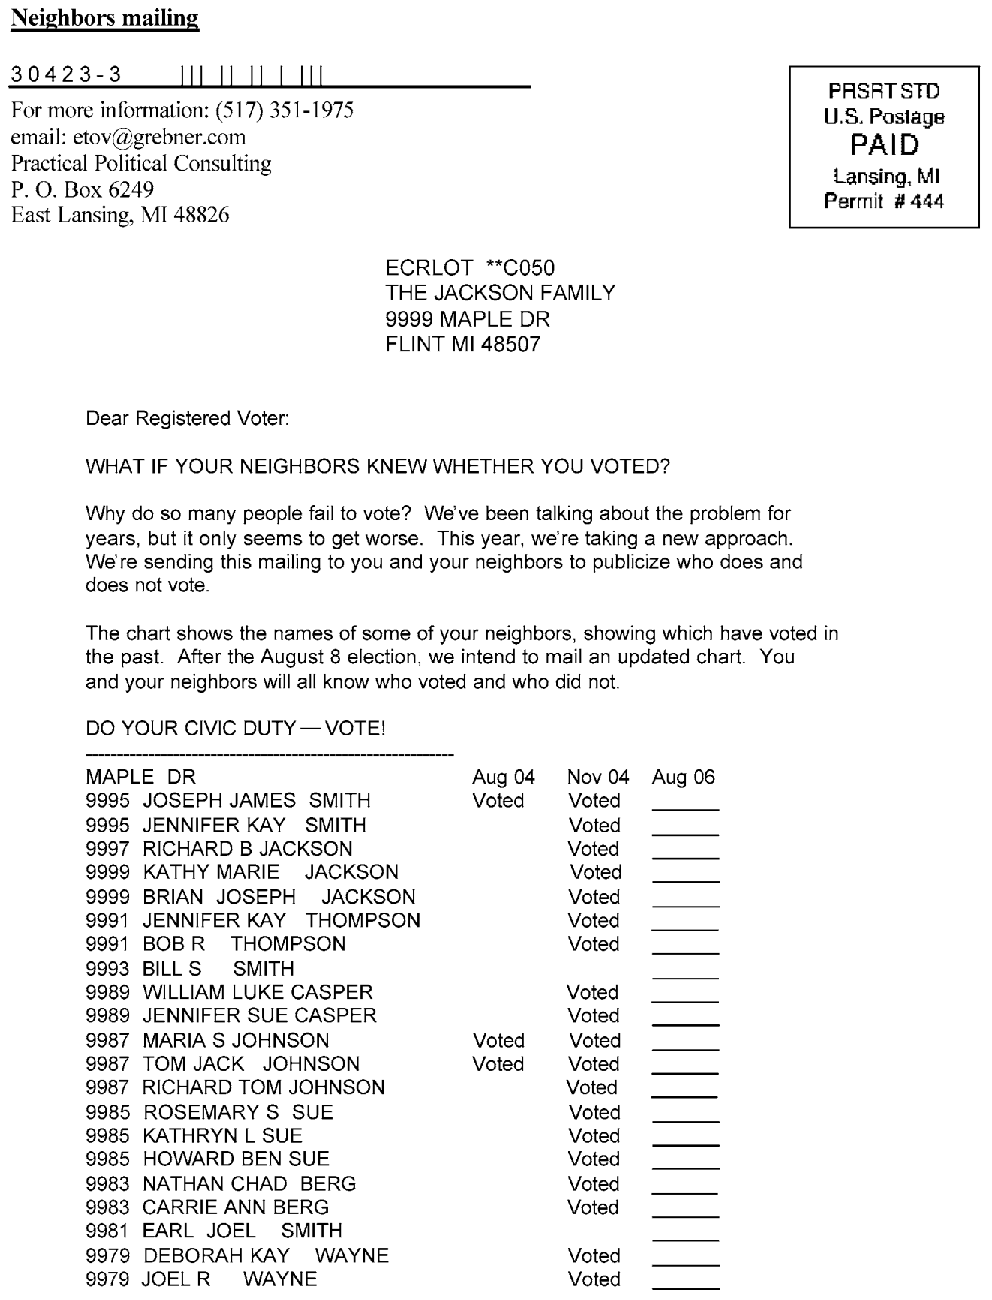
\includegraphics[height=0.74\textheight]{gerber_mailing.pdf}

  \slidesource{The ``Neighbors'' mailing, Gerber, Green \& Larimer (2008) replication archive, doi:10.60600/YU/CGMWNW (CC0)}
\end{frame}


\begin{frame}[fragile]
\frametitle{Example: Social Pressure Experiment}
\small
\begin{Verbatim}[fontsize=\scriptsize, frame=single, label=R Code, commandchars=\\\{\}]
> mod1 <- lm(voted~Tr_Hawthorne+Tr_CivicDuty+Tr_Neighbors+Tr_Self,data=dta)
> coeftest(mod1) # \alert{homoskedastic}
t test of coefficients:
               Estimate Std. Error t value  Pr(>|t|)
(Intercept)   0.3076541  0.0052062 59.0935 < 2.2e-16 ***
Tr_Hawthorne  0.0237709  0.0128791  1.8457   0.06496 .
Tr_CivicDuty -0.0044725  0.0127744 -0.3501   0.72626
Tr_Neighbors  0.0718986  0.0129031  5.5722 2.561e-08 ***
Tr_Self       0.0502013  0.0127711  3.9308 8.505e-05 ***
\end{Verbatim}
In this subset (14,392 voters), the intra household error correlation is estimated at $\hat\rho=.50$ (.53 in the full sample of 344,084 voters) \\ \medskip
This suggests that treating voters within the same household as independent is unrealistic
(i.e., about half of the error variance comes from a component shared by everyone in the household)
\end{frame}





\begin{frame}[fragile]
\frametitle{Example: Social Pressure Experiment}
\small
\begin{Verbatim}[fontsize=\scriptsize, frame=single, label=R Code, commandchars=\\\{\}]
> mod1 <- lm(voted~Tr_Hawthorne+Tr_CivicDuty+Tr_Neighbors+Tr_Self,data=dta)
> coeftest(mod1) # \alert{homoskedastic}
t test of coefficients:
               Estimate Std. Error t value  Pr(>|t|)
(Intercept)   0.3076541  0.0052062 59.0935 < 2.2e-16 ***
Tr_Hawthorne  0.0237709  0.0128791  1.8457   0.06496 .
Tr_CivicDuty -0.0044725  0.0127744 -0.3501   0.72626
Tr_Neighbors  0.0718986  0.0129031  5.5722 2.561e-08 ***
Tr_Self       0.0502013  0.0127711  3.9308 8.505e-05 ***
>
> coeftest(mod1, vcov = vcovCL(mod1, cluster = ~ hh_id)) # \alert{clustered}
t test of coefficients:
               Estimate Std. Error t value  Pr(>|t|)
(Intercept)   0.3076541  0.0063711 48.2894 < 2.2e-16 ***
Tr_Hawthorne  0.0237709  0.0157746  1.5069  0.131857
Tr_CivicDuty -0.0044725  0.0154991 -0.2886  0.772917
Tr_Neighbors  0.0718986  0.0164533  4.3699 1.252e-05 ***
Tr_Self       0.0502013  0.0162195  3.0951  0.001971 **
\end{Verbatim}
CR standard errors are 21--28\% larger than homoskedastic
\end{frame}

\begin{frame}
\frametitle{Example: Large Clusters, a Regressor Assigned by Region}
\small
\begin{itemize}
\item British Election Study, May--June 2016: 16,331 respondents in 167 NUTS-3 regions (98 per region on average).
\item $Y = 1$ if the respondent intends to vote Leave. $X$ = the Chinese import shock of the respondent's region, the same for everyone in it. Both models control for age and gender.
\end{itemize}
\medskip
\begin{center}
\begin{tabular}{lccccc}
\hline
 & $\hat\beta_{shock}$ & Classical SE & Clustered SE & Ratio & $\hat\rho$ \\
\hline
Without region dummies & 0.279 & 0.029 & 0.067 & 2.3 & .03 \\
With NUTS-1 region dummies (11 regions) & 0.154 & 0.032 & 0.039 & 1.2 & .01 \\
\hline
\end{tabular}
\end{center}
\medskip
\pause
\begin{itemize}
\item $\hat\rho = .03$ is small, but the clusters are large. With 98 respondents per region, it is enough to more than double the SE.
\item The ratio falls because people in one part of Britain share regional factors and shocks (for example, Scotland's political culture). The first model leaves them in the error. The region dummies absorb them, so little correlation is left within NUTS-3 regions.
\end{itemize}
\slidesource{Colantone \& Stanig (2018), \emph{APSR} 112(2), individual data (BES wave 8, 2016); linear probability model, SEs clustered by NUTS-3 region}
\end{frame}


\frame{
\frametitle{Cluster Robust Standard Errors (CRSE)}
\small
\begin{itemize}
\item CRSE do not change our estimate $\hat{\b}$ and do not fix potential bias in $\hat{\b}$
\item CRSE are consistent estimators for $V[\hat{\b}]$ given cluster dependence (i.e. independence across clusters, dependence within)
    \begin{itemize}
      \item How much larger CRSE are depends on the within-cluster correlation of both the errors and the regressor, and on cluster size (21--28\% for the letters, 2.3 times for the Brexit survey)
      \item \alert{Always use CRSE if you suspect cluster dependence, unless number of clusters is small}
    \end{itemize}
\item Performance of CRSE depends on number of clusters. With too few clusters, CRSE are not valid and often downward biased
    \begin{itemize}
      \item There is no safe cutoff: depending on the setting, ``few'' can mean fewer than 20 to fewer than 50 balanced clusters (Cameron and Miller 2015).
      \item A simulation-based method called the wild cluster bootstrap can be used
      if number of clusters is too small (450C and D)

%     Cameron, A. Colin, Gelbach, Jonah B. and Miller, Douglas L. (2008). ?Bootstrap-
%Based Improvements for Inference with Clustered Errors?, The Review of Economics and
%Statistics 90(3), 414?427.
    \end{itemize}
\end{itemize}
}

%\frame{
%\frametitle{Cluster Robust Standard Errors (CRSE) \& Fixed Effects}
%\small
%\begin{itemize}
%\item Without fixed effects:
%    \begin{itemize}
%      \item Need clustering if clustering in sampling and hetergenous treatment effects \emph{or}
%      \item Need clustering if clustering in assignment
%    \end{itemize}
%\item With fixed effects:
%    \begin{itemize}
%      \item Need clustering if clustering in sampling and hetergenous treatment effects \emph{or}
%      \item Need clustering if clustering in assignment and heterogenous treatment effects
%    \end{itemize}
%\end{itemize}
%}


\section{Serial Correlation}

\frame{
\frametitle{Time Dependence: Serial Correlation}
\small
Suppose we observe a unit at multiple times $t=1,...,T$ (e.g. a country over several years, an individual over several months, etc.).\\\bigskip

Such observations are often \alert{serially correlated} (not independent across time). We can model this with the following \alert{AR(1) model}:
$$
y_{t} = \beta_0 + \beta_1 x_{t}  +u_{t}
$$
where the \alert{autoregressive error} is $$
u_t=\rho\, u_{t-1}+e_{t} \quad \mbox{where} \quad |\rho|<1
$$
\begin{itemize}\pause
  \item $e_t \sim N(0, \sigma^2_e)$\pause
  \item $\rho$ is an unknown \alert{autoregressive coefficient}  (note if $\rho=0$ we have classic errors used before) \pause
  \item Typically assume stationarity meaning that $V[u_t]$ and $Cov[u_t,u_{t+h}]$ are independent of $t$
\item Generalizes to higher order serial correlation (e.g. an AR(2) model is given by $u_t=\rho u_{t-1}+\delta u_{t-2}+e_{t}$).
\end{itemize}

}

\frame{
\frametitle{The Error Structure for the AR(1) Model}
\small
We have $\mb{u}=\left[
\begin{array}{cccc}
  u_1 & u_2 & ... & u_T
\end{array}\right]'
$
and the AR(1) model implies the following error structure:

$$
V[\mb{u}]=\Sig = \frac{\sigma_e^2}{(1-\rho^2)}\left[ \begin{array}{ccccc} 1   & \rho &  \rho^2 &  \dots & \rho^{T-1} \\
%V[\mb{u}]=\Sig =\sigma^2 \left[ \begin{array}{ccccc} 1   & \rho &  \rho^2 &  \dots & \rho^{T-1} \\
\rho& 1  & \rho & \dots & \rho^{T-2}  \\
\rho^2& \rho  & 1 & \dots & \rho^{T-3}  \\
 \vdots & \vdots & \vdots &  \ddots & \vdots\\
 \rho^{T-1} & \rho^{T-2} & \rho^{T-3}  & \dots& 1 \end{array} \right]
$$

That is, the covariance between errors in $t=1$ and $t=2$ is $\frac{\sigma_e^2}{(1-\rho^2)} \rho$, between errors in $t=1$ and $t=3$ is $\frac{\sigma_e^2}{(1-\rho^2)} \rho^2$, etc. \\ \medskip
This implies that the correlation between the errors decays exponentially with the number of periods separating them. \\
\pause
\bigskip

$\rho$ is usually positive. If the regressor is also positively autocorrelated, as most time series are, ignoring serial correlation makes the conventional standard errors too small.

}


\frame{
\frametitle{Derivation of Error Structure for the AR(1) Model}
\small

We have
$$
V[u_t]=V[\rho u_{t-1}+e_{t}]=\rho^2V[u_{t-1}]+\sigma_e^2
$$
with stationarity, $V[u_t]=V[u_{t-1}]$, and so
$$
V[u_t](1-\rho^2)=\sigma_e^2 \Rightarrow V[u_t]=\frac{\sigma_e^2}{(1-\rho^2)}
$$
also

$$
Cov[u_t,u_{t-1}]=E[u_t u_{t-1}]=E[(\rho u_{t-1} + e_{t})u_{t-1}]=\rho V[u_{t-1}]=\rho \frac{\sigma_e^2}{(1-\rho^2)}
$$
or generally
$$
Cov[u_t,u_{t-h}]=\rho^h \frac{\sigma_e^2}{(1-\rho^2)}
$$


}






\frame{
\frametitle{How to Detect and Fix Serially Correlated Errors}
\small
Detection:
\begin{itemize}
\item Plot residuals over time (or more fancy ``autocorrelation'' plots)
\item Formal tests (e.g. Durbin-Watson statistics)
\end{itemize}

\vspace{.5cm}
\pause
Possible Corrections:
\begin{itemize}
\item Use standard errors that are robust to serial correlation (e.g. Newey-West)
\item AR corrections (e.g. Prais-Winsten, Cochrane-Orcutt, etc.)
\item Lagged dependent variables or other dynamic panel models
\item First-differencing the data
\end{itemize}

}

\frame{
\frametitle{Monthly Approval and Business Expectations}

{\centering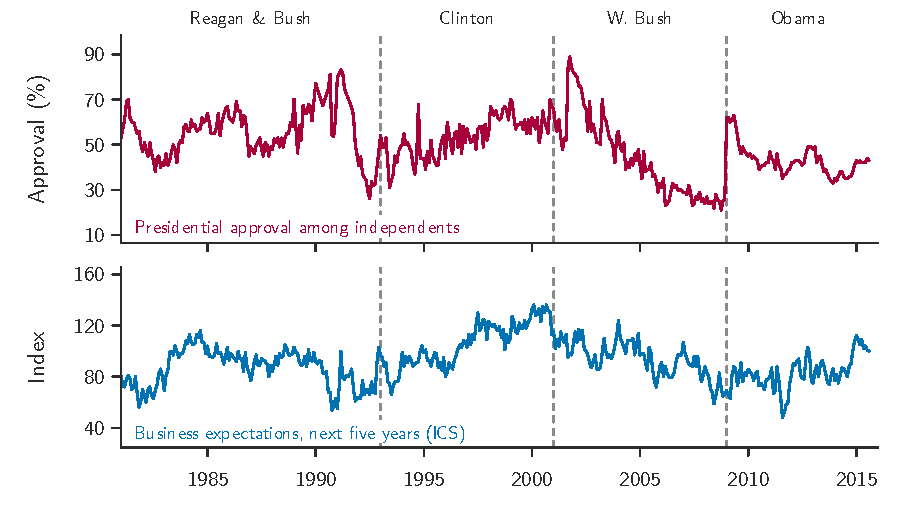
\includegraphics[height=0.78\textheight]{donovan_series.pdf}\par}
\slidesource{Donovan, Kellstedt, Key \& Lebo (2020), \emph{Political Behavior} 42(4); monthly, Jan.~1981--Aug.~2015. Dashed lines: a new administration.}

}


\begin{frame}[fragile]
\frametitle{Monthly Approval and Business Expectations}

\begin{Verbatim}[fontsize=\footnotesize, frame=single, label=R Code, commandchars=\\\{\}]
> mod1 <- lm(ind ~ bus5yr + clinton + gwb + obama, data=dta)
> coeftest(mod1)

t test of coefficients:

              Estimate Std. Error t value  Pr(>|t|)
(Intercept)  27.615771   3.319727  8.3187 1.323e-15 ***
bus5yr        0.324423   0.036757  8.8262 < 2.2e-16 ***
clinton      -8.299574   1.597577 -5.1951 3.228e-07 ***
gwb         -14.148390   1.465549 -9.6540 < 2.2e-16 ***
obama       -11.392846   1.531328 -7.4398 5.943e-13 ***
\end{Verbatim}
{\footnotesize \texttt{ind}: approval among independents (\%); \texttt{bus5yr}: expected business conditions over the next five years (Index of Consumer Sentiment); \texttt{clinton}, \texttt{gwb}, \texttt{obama}: administration dummies (Reagan and G.~H.~W. Bush are the baseline).}
\end{frame}


\frame{
\frametitle{Tests for Serial Correlation: Durbin-Watson}
Recall our AR(1) model is:
$$
y_{t} = \beta_0 + \beta_1 x_{t}  +u_{t}
$$
where $u_t=\rho u_{t-1}+e_{t}$, $e_t \sim N(0, \sigma_e^2)$, and $\rho$ is our unknown \alert{autoregressive coefficient} (with $|\rho|<1$).\\\bigskip \pause

The null hypothesis (no serial correlation) is: $H_0$: $\rho=0$ \\
The alternative (positive serial correlation): $H_1$: $\rho>0$\\ \bigskip

One common test for serial correlation is the \alert{Durbin-Watson statistic}

%In Stata: \texttt{estat dwatson}

}

\frame{
\frametitle{(Optional) Tests for Serial Correlation: Durbin-Watson}

$$
DW=\frac{\sum_{t=2}^{T} (\hat{u}_t - \hat{u}_{t-1})^2}{\sum_{t=1}^{T} \hat{u}_t^2} \quad \mbox{where} \quad DW\approx2(1-\widehat{\rho})
$$\pause
\[
DW - 2(1 - \hat{\rho}) = -\frac{\hat{u}_1^2 + \hat{u}_T^2}{\sum_{t=1}^{T}\hat{u}_t^2} \xrightarrow{p} 0,
\]
where $\hat{\rho} = \frac{\sum_{t=2}^{T}\hat{u}_t\hat{u}_{t-1}}{\sum_{t=1}^{T}\hat{u}_t^2}$ is the first-order sample autocorrelation of the residuals.
Since $\hat{\rho} \xrightarrow{p} \rho$, the Durbin–Watson statistic converges in probability to $2(1-\rho)$ as $T\to\infty$.\\ \medskip

Rules of thumb (the test's exact critical values depend on $T$ and $k$):
\begin{itemize}
\item If $DW\approx2$ then $\widehat{\rho}\approx0$
\item If $DW<1$ we have serious positive serial correlation
\item If $DW>3$ we have serious negative serial correlation
\end{itemize}
}

% \frame{
% \frametitle{Tests for Serial Correlation: Durbin-Watson}

% $$
% DW=\frac{\sum_{t=2}^{n} (\hat{u}_t - \hat{u}_{t-1})^2}{\sum_{t=1}^{n} \hat{u}_t^2} \quad \mbox{where} \quad DW\approx2(1-\widehat{\rho})
% $$\pause\medskip

% \textbf{Worksheet Q3} Show
% \[
% DW \xrightarrow{p} 2(1 - \hat{\rho}),
% \]
% where $\hat{\rho} = \frac{\sum_{t=2}^{T}\hat{u}_t\hat{u}_{t-1}}{\sum_{t=1}^{T}\hat{u}_t^2}$ is the sample autocorrelation of the residuals (the OLS estimate of $\rho$).  
% In other words, as $T\to\infty$, the Durbin–Watson statistic converges in probability to $2(1-\hat{\rho})$. Explain:
% \begin{itemize}
% \item If $DW\approx2$ then $\widehat{\rho}\approx0$
% \item If $DW<1$ we have serious positive serial correlation
% \item If $DW>3$ we have serious negative serial correlation
% \end{itemize}
% }



\begin{frame}[fragile]
\frametitle{Monthly Approval and Business Expectations}

\begin{Verbatim}[fontsize=\footnotesize, frame=single, label=R Code, commandchars=\\\{\}]
> library(lmtest)
> dwtest(mod1)

	Durbin-Watson test

data:  mod1
DW = 0.32152, p-value < 2.2e-16
alternative hypothesis: true autocorrelation is greater than 0
\end{Verbatim}
The test rejects no serial correlation: the residuals are strongly positively autocorrelated ($\hat\rho \approx 0.84$). Business expectations are also strongly autocorrelated (0.90 from one month to the next), so the conventional standard errors are likely far too small.
\end{frame}


%
%\frame{
%\frametitle{Corrections: Prais Winston}
%
%One way to correct for serial correlation is to run OLS on \alert{quasi-differenced data} where we transform the original data to eliminate serial correlation (this is called \alert{pre-whitening}):
%\begin{align*}
%y_{t-1} &= \beta_0 + \beta_1 x_{t-1} + u_{t-1} \\
%y_t &= \beta_0 + \beta_1 x_{t} + u_{t}
%\end{align*}
%Multiply the first equation by $\rho$ and subtract it from the second:
%$$
%\tilde{y}_t = (1-\rho)\beta_0 + \beta_1 \tilde{x}_t + e_t
%$$
%where $\tilde{y}_t=y_t-\rho y_{t-1}$ and $\tilde{x}_t=x_t - \rho x_{t-1}$.\\\bigskip\pause
%
%We usually estimate $\rho$ with a regression of $\hat{u}_t$ on $\hat{u}_{t-1}$ and rely on an iterative scheme where the data is differenced until serial correlation is eliminated. This FGLS scheme is called: \alert{Prais-Winston estimation} (\texttt{prais y x}).
%
%}
%

\frame{
\frametitle{Corrections: HAC Standard Errors}

\begin{itemize}
  \item A common way to correct for serial correlation is to use OLS but to estimate the variances using an estimator that is \alert{heteroskedasticity and autocorrelation consistent (HAC)}
(Newey and West 1987).\bigskip
  \item The theory behind the HAC variance estimator is somewhat complicated, but the interpretation is similar to our usual OLS robust standard errors.\medskip
  \begin{itemize}
  \addtolength{\itemsep}{.5\baselineskip}
    \item HAC standard errors leave estimate of $\hat{\b}$ unchanged and do not fix potential bias in $\hat{\b}$
\item HAC estimators are consistent for $V[\hat{\b}]$ under heteroskedasticity and/or autocorrelation as $T$ grows, if the number of lags used grows slowly with $T$
    \item The \texttt{sandwich} package in R implements a variety of HAC estimators

    \item A common option is \texttt{NeweyWest}; by default it chooses the number of lags from the data and applies a prewhitening step to the regressor-times-residual terms (see \texttt{?NeweyWest}). Without that step, the slope's SE on the next slide would be 0.075 instead of 0.079
  \end{itemize}
\end{itemize}

}


\begin{frame}[fragile]
\frametitle{Monthly Approval and Business Expectations}

\begin{Verbatim}[fontsize=\scriptsize, frame=single, label=R Code, commandchars=\\\{\}]
> coeftest(mod1) # \alert{homoskedastic errors}
t test of coefficients:
              Estimate Std. Error t value  Pr(>|t|)
(Intercept)  27.615771   3.319727  8.3187 1.323e-15 ***
bus5yr        0.324423   0.036757  8.8262 < 2.2e-16 ***
clinton      -8.299574   1.597577 -5.1951 3.228e-07 ***
gwb         -14.148390   1.465549 -9.6540 < 2.2e-16 ***
obama       -11.392846   1.531328 -7.4398 5.943e-13 ***

> coeftest(mod1, vcov = NeweyWest) # \alert{HAC errors}
t test of coefficients:
              Estimate Std. Error t value  Pr(>|t|)
(Intercept)  27.615771   8.791195  3.1413  0.001804 **
bus5yr        0.324423   0.078904  4.1116 4.747e-05 ***
clinton      -8.299574   2.927949 -2.8346  0.004815 **
gwb         -14.148390   6.244890 -2.2656  0.023996 *
obama       -11.392846   4.647416 -2.4514  0.014644 *
\end{Verbatim}
Once we correct for autocorrelation, the slope's standard error is 2.1 times as large (0.079 instead of 0.037). The slope is still clearly positive ($t = 4.1$).
\end{frame}

\begin{frame}[fragile]
\frametitle{First Differences: Is the Link Month to Month?}
\small
\begin{itemize}
\item HAC fixes the standard errors, not a spurious trend. Two series that drift slowly together give a large slope in levels even if their month-to-month changes are unrelated.
\item First differences check whether the link is month to month. We regress the change in approval on the change in business expectations.
\end{itemize}
\begin{Verbatim}[fontsize=\scriptsize, frame=single, label=R Code, commandchars=\\\{\}]
> mod_fd <- lm(d_ind ~ d_bus + d_clinton + d_gwb + d_obama, data = fd)
> coeftest(mod_fd)
             Estimate Std. Error t value  Pr(>|t|)
(Intercept) -0.130212   0.277004 -0.4701   0.63855
d_bus        0.077375   0.036214  2.1366   0.03322 *
...
\end{Verbatim}
\pause
\begin{itemize}
\item The slope shrinks from 0.32 to 0.077. With the usual SE, $t = 2.1$. With the Newey-West SE (computed without prewhitening, which fails for this model), $t = 1.9$, just short of the 5\% cutoff (1.96). So the month-to-month link is positive but small, and not clearly different from zero. It is much weaker than the slope in levels. The data do not tell us why: the two series may drift together for other reasons, approval may take more than a month to respond, or monthly changes in a survey index may be mostly noise, which pulls the slope toward zero.
\end{itemize}
\end{frame}



%


\section{Summary}

\frame{
\frametitle{Summary}
\small
\begin{itemize}
  \item Non-constant error variance and correlated errors can make conventional standard errors badly wrong, even if the estimates of the regression coefficients are unbiased
  \begin{itemize}
    \item Heteroskedasticity
    \item Clustering
    \item Serial correlation
  \end{itemize}
  \item Both can be detected with plots or formal tests.
  \item A common approach is simply to always use robust standard errors unless $n$ or the number of clusters $M$ is too small
        \begin{itemize}
    \item White standard errors
    \item Cluster robust standard errors
    \item Newey-West HAC standard errors
  \end{itemize}
\end{itemize}

}

\end{document}
